\part{Segundo semestre}

\chapterimage{3.pdf} % Chapter heading image

\chapter{Cálculo Multivariado}


\section{Espacio Vectorial}

\begin{definition}[Vector]
	Es un elemento del espacio vectorial
\end{definition}

Un espacio vectorial es un conjunto no vacío, dotado de dos operaciones binarias:

\begin{itemize}
	\item Suma
	\item Producto por escalar
\end{itemize}

Son las estructuras que conforman a los \textbf{grupos}, \textbf{anillos} y \textbf{campos} y satisfacen los siguientes axiomas:

\subsection{Axiomas para sumar escalares:}

\begin{enumerate}
	\item Sean $x,y\in V$ (el conjunto no vacío) $\implies x+y\in V$ (propiedad de cerradura)
	\item Sean $x,y\in V\implies x+y=y+x\quad \forall x,y\in V$ (propiedad de conmutatividad)
	\item Sean $x,y,z\in V\implies x+(y+z)=(x+y)+z\quad \forall x,y,z\in V$ (Propiedad asociativa)
	\item $\exists \bar{0}\in V \in x+\bar{0}=x=\bar{0}+x\quad \forall x\in V$ (Propiedad del neutro aditivo)
	\item $\forall x\in V \exists -x\in V \in -x+x=\bar{0}$ y $x+(-x)=\bar{0}$ (Propiedad del inverso aditivo)
\end{enumerate}

\subsection{Axiomas para multiplicación por escalar:}

\begin{enumerate}
	\item Si $x\in V\implies ax\in V \quad \forall a\in K (K=\R)$
	\item $a(x+y)=ax+ay\quad \forall x,y\in V$ y $a\in\R$
	\item $a(bx)=(ab)x\quad \forall x\in V$ y $a,b\in \R$
	\item $1\cdot x=x\quad \forall x\in V$
\end{enumerate}

\begin{example}
	Sea $B$ el conjunto de polinomios de grado $n=2$ verifique si este conjunto forma un espacio vectorial con las operaciones de suma y producto por escalar usuales:
\end{example}

\textit{ Sol. }

\begin{align*}
	 & V=\left\{ a_2x^2+a_1x+a_0\mid a_2,a_1,a_0\in\R \right\}                     \\
	 & \text{Sea } P(x)\text{ y } Q(x)\in V\implies P(x)+Q(x)=                     \\
	 & \left(p-2x^2+p_1x+p_0\right)+\left(q_2x^2+q_1x+q_0\right)=                  \\
	 & \left(p_2+q_2\right)x^2+\left(p_1+q_1\right)x+\left(p_0+q_0\right)=(P+Q)(x)
\end{align*}

Para el producto escalar se necesita un campo:

\begin{align*}
	 & \text{Sea } Q(x)\in V \text{ y } a\in\R\implies aQ(x)=   \\
	 & a\left(q_1x^2+q_1x+q_0\right)=aq_2x^2+aq_1x+aq_0=(aQ)(x)
\end{align*}

Sean $p(x)=x^2+2x+1$ y $q(x)=-x^2+2$ aplicando los axiomas, se pueden sumar las funciones:
\begin{align*}
	 & p(x)+q(x)=(1+(-1))x^2+2x+(1+2)                     \\
	 & =(1-1)x^2+2x+3                                     \\
	 & =2x+3\to \text{Es un polinomio de grado 1}\notin V
\end{align*}

Como no se satisface la propiedad de cerradura, por lo tanto el conjunto $V$ con las operaciones de suma y producto
por escalar de polinomio usuales, no forman un espacio vectorial.


\begin{problem}[Sean $x,y\in M_{2\times 2}(\R)$ se define la suma usual de matrices como:]
\begin{equation}
	a+b=\begin{bmatrix}a_{11}&a_{12}\\a_{21}&a_{22}\end{bmatrix}+\begin{bmatrix}b_{11}&b_{12}\\b_{21}&b_{22}\end{bmatrix}=\begin{bmatrix}a_{11}+b_{11}&a_{12}+b_{12}\\a_{21}+b_{21}&a_{22}+b_{22}\end{bmatrix}
\end{equation}
\end{problem}

\textit{ Sol. }

\textbf{OPERACIÓN SUMA}

\begin{exercise}[Propiedad de cerradura de la suma en el conjunto]
	Sean $A$ y $B\in V=M_{2\times 2}(\R)$ entonces
\end{exercise}

\begin{align*}
	 & A+B=\begin{pmatrix}
		       a_{11} & a_{12} \\a_{21}&a_{22}
	       \end{pmatrix}+\begin{pmatrix}
		                     b_{11} & b_{12} \\b_{21}&b_{22}
	                     \end{pmatrix}=\begin{pmatrix}
		                                   a_{11}+b_{11} & a_{12}+a_{12} \\a_{21}+b_{21}&a_{22}+b_{22}
	                                   \end{pmatrix} \\
	 & \text{Con esto se verifica que la operación suma es cerrada en }                           \\
	 & V=M_{2\times 2}(\R)
\end{align*}

\begin{exercise}[Verifique que $x+y=y+x$, Sean]

	$x=\begin{pmatrix}
			x_{11} & x_{12} \\x_{21}&x_{22}
		\end{pmatrix},y=\begin{pmatrix}y_{11} & y_{12} \\y_{21}&y_{22}
		\end{pmatrix}\in M_{2\times 2}(\R)$
\end{exercise}

\textit{ Sol. }

\begin{align*}
	 & \text{Sea: }=\begin{pmatrix}
		                x_{11} & x_{12} \\x_{21}&x_{22}
	                \end{pmatrix},y=\begin{pmatrix}y_{11} & y_{12} \\y_{21}&y_{22}
	                                \end{pmatrix}                 \\
	 & x+y=\begin{pmatrix}
		       x_{11} & x_{12} \\x_{21}&x_{22}
	       \end{pmatrix}+\begin{pmatrix}
		                     y_{11} & y_{12} \\y_{21}&y_{22}
	                     \end{pmatrix}=\begin{pmatrix}
		                                   x_{11}+y_{11} & x_{12}+y_{12} \\x_{21}+y_{21}&x_{22}+y_{22}
	                                   \end{pmatrix} \\
	 & \begin{pmatrix}
		   y_{11}+x_{11} & y_{12}+x_{12} \\y_{21}+x_{21}&y_{22}+x_{22}
	   \end{pmatrix}=\begin{pmatrix}
		                 y_{11} & y_{12} \\y_{21}&y_{22}
	                 \end{pmatrix}+\begin{pmatrix}
		                               x_{11} & x_{12} \\x_{21}&x_{22}
	                               \end{pmatrix}
\end{align*}
La conmutabilidad con la suma si se da en este conjunto.

\begin{exercise}[Sean: $x=\begin{pmatrix}
				x_{11} & x_{12} \\x_{21}&x_{22}
			\end{pmatrix},y=\begin{pmatrix}y_{11} & y_{12} \\y_{21}&y_{22}
			\end{pmatrix}, z=\begin{pmatrix}z_{11} & z_{12} \\z_{21}&z_{22}
			\end{pmatrix}\in M_{2\times 2}(\R)$]

	\begin{align*}
		 & x+(y+z)=\begin{pmatrix}
			           x_{11} & x_{12} \\x_{21}&x_{22}
		           \end{pmatrix}+\left[\begin{pmatrix}y_{11} & y_{12} \\y_{21}&y_{22}
			                               \end{pmatrix}+\begin{pmatrix}z_{11} & z_{12} \\z_{21}&z_{22}
			                                             \end{pmatrix}\right]=                                     \\
		 & =\begin{pmatrix}
			    x_{11} & x_{12} \\x_{21}&x_{22}
		    \end{pmatrix}+\begin{pmatrix}
			                  x_{11}+z_{11} & x_{12}+z_{12} \\x_{21}+z_{21}&x_{22}+z_{22}
		                  \end{pmatrix}=\begin{pmatrix}
			                                x_{11}+(z_{11}+z_{11}) & x_{12}+(y_{12}+z_{12}) \\x_{21}+(y_{21}+z_{21})&x_{22}+(z_{22}+z_{22})
		                                \end{pmatrix} \\
		 & =\begin{pmatrix}
			    x_{11}+z_{11}+z_{11} & x_{12}+y_{12}+z_{12} \\x_{21}+y_{21}+z_{21}&x_{22}+z_{22}+z_{22}
		    \end{pmatrix}=\begin{pmatrix}
			                  (x_{11}+z_{11})+z_{11} & (x_{12}+y_{12})+z_{12} \\(x_{21}+y_{21})+z_{21}&(x_{22}+z_{22})+z_{22}
		                  \end{pmatrix}               \\
		 & =\left[\begin{pmatrix}
				          x_{11} & x_{12} \\x_{21}&x_{22}
			          \end{pmatrix}+\begin{pmatrix}y_{21} & y_{22}
			                        \end{pmatrix}\right]+\begin{pmatrix}z_{21} & z_{22}
		                                             \end{pmatrix}=(x+y)+z
	\end{align*}

	La operación suma en este conjunto es asociativa
\end{exercise}

\begin{exercise}[Espacio vectorial, sea:]
	\begin{equation*}
		\bar{0}=\begin{pmatrix}
			0_{11} & 0_{12} \\0_{21}&0_{22}
		\end{pmatrix}, \bar{x}=\begin{pmatrix}
			\bar{x}_{11} & \bar{x}_{12} \\ \bar{x}_{21}&\bar{x}_{22}
		\end{pmatrix}\in M_{2\times 2}(\R)
	\end{equation*}

	Por verificar que $x+\bar{0}=x=\bar{0}+x$

	\textit{ Sol. }
	\begin{align*}
		 & x+\bar{0}=\begin{pmatrix}
			             x_{11} & x_{12} \\x_{21}&x_{22}
		             \end{pmatrix}+\begin{pmatrix}
			                           0_{11} & 0_{12} \\0_{21}&0_{22}
		                           \end{pmatrix} &  & =\begin{pmatrix}
			                                               x_{11} & x_{12} \\x_{21}&x_{22}
		                                               \end{pmatrix}\begin{pmatrix}
			                                                            x_{11}+0_{11} & x_{12}+0_{12} \\x_{21}+0_{21}&x_{22}+0_{22}
		                                                            \end{pmatrix} \\
		 & \implies x_{11}+0_{11}=x_{11}   &  & ;x_{21}+0_{21}=x_{12}                                                          \\
		 & x_{12}+0_{12}=x_{12}            &  & ;x_{22}+0_{22}=x_{22}                                                          \\
		 & \implies 0_{11}=x_{11}-x_{11}   &  & ;0_{21}=x_{21}-x_{21}                                                          \\
		 & 0_{12}=x_{12}-x_{12}            &  & ;0_{22}=x_{22}-x_{22}                                                          \\
		 & \implies 0_{11}=0               &  & ;0_{21}=0                                                                      \\
		 & 0_{12}=0                        &  & ; 0_{22}=0                                                                     \\
		 &                                 &  & \therefore \bar{0}=\begin{pmatrix}
			                                                           0 & 0 \\0&0
		                                                           \end{pmatrix}\in M_{2\times 2}(\R)                          \\
		 & x+\bar{0}=\begin{pmatrix}
			             x_{11} & x_{12} \\x_{21}&x_{22}
		             \end{pmatrix}+\begin{pmatrix}
			                           0 & 0 \\0&0
		                           \end{pmatrix} &  & =\begin{pmatrix}
			                                               x_{11}+0 & x_{12}+0 \\x_{21}+0&x_{22}+0
		                                               \end{pmatrix}=\begin{pmatrix}
			                                                             x_{11} & x_{12} \\x_{21}&x_{22}
		                                                             \end{pmatrix}=x
	\end{align*}
	Ahora falta comprobar que $\bar{0}+x=x$, se verificará la unicidad del cero testado $\bar{0}$, para ello se supondrá que hay otro elemento en $M_{2\times 2}(\R)$ que tiene la misma propiedad, es decir: $x+\hat{0}=x=x+\bar{0}$

	\begin{align*}
		 & \implies x+\hat{0}=(x+\bar{0})+\hat{0}=x                                                                \\
		 & \left[\begin{pmatrix}
				         x_{11} & x_{12} \\ x_{21}&x_{22}
			         \end{pmatrix}+\begin{pmatrix}
				                       0 & 0 \\0&0
			                       \end{pmatrix}\right]+\begin{pmatrix}
			                                            \hat{0}_{11} & \hat{0}_{12} \\ \hat{0}_{21}&\hat{0}_{22}
		                                            \end{pmatrix}=\begin{pmatrix}
			                                                          x_{11} & x_{12} \\x_{21}&x_{22}
		                                                          \end{pmatrix}        \\
		 & \implies \begin{pmatrix}
			            x_{11}+0 & x_{12}+0 \\x_{21}+0&x_{21}+0
		            \end{pmatrix}+\begin{pmatrix}
			                          \hat{0}_{11} & \hat{0}_{12} \\ \hat{0}_{21}&\hat{0}_{22}
		                          \end{pmatrix}=                          \\
		 & \begin{pmatrix}
			   x_{11} & x_{12} \\x_{21}&x_{21}
		   \end{pmatrix}\begin{pmatrix}
			                x_{11}+0+\hat{0}_{11} & x_{12}+0+\hat{0}_{12} \\x_{21}+0+\hat{0}_{21}&x_{21}+0+\hat{0}_{22}
		                \end{pmatrix}=\begin{pmatrix}
			                              x_{11} & x_{12} \\x_{21}&x_{21}
		                              \end{pmatrix} \\
		 & x_{11}+0+\hat{0}_{11}=x_{11}\implies 0+\hat{0}_{11}=x_{11}-x_{11}                                       \\
		 & x_{12}+0+\hat{0}_{12}+x_{12}\implies 0+\hat{0}_{12}=x_{12}-x_{12}                                       \\
		 & x_{21}+0+\hat{0}_{21}=x_{21}\implies 0+\hat{0}_{21}=x_{21}-x_{21}                                       \\
		 & x_{22}+0+\hat{0}_{22}=x_{22}\implies 0+\hat{0}_{22}=x_{22}-x_{22}
	\end{align*}
\end{exercise}

\begin{exercise}[Sea $x\in M_{2\times 2}(\R)x^{-1}$ denotado así el inverso aditivo, tal que $x^{-1}\in M_{2\times 2}(\R)$ que cumple con la propiedad de que: $x+x^{-1}=\bar{0}$]
	\begin{align*}
		 & x+x^{-1}=\begin{pmatrix}
			            x_{11}+x_{12} \\x_{21}+x_{22}
		            \end{pmatrix}+\begin{pmatrix}
			                          x^{-1}_{11}+x^{-1}_{12} \\x^{-1}_{21}+x^{-1}_{22}
		                          \end{pmatrix}=\begin{pmatrix}
			                                        0 & 0 \\0&0
		                                        \end{pmatrix} \\
		 & \implies x_{11}+x^{-1}_{11}=0 \implies +x^{-1}_{11}=0-x_{11}            \\
		 & x_{12}+x^{-1}_{12}=0\implies x^{-1}_{12}=0-x_{12}                       \\
		 & x_{21}+x^{-1}_{21}=0\implies x^{-1}_{21}=0-x_{21}                       \\
		 & x_{22}+x^{-1}_{22}=0\implies x^{-1}_{22}=0-x_{22}
	\end{align*}

	Ahora por igualdad sabemos que:
	\begin{align*}
		                    & x^{-1}_{11}=-x_{11} &   &
		x^{-1}_{12}=-x_{12} &                     &
		x^{-1}_{21}=-x_{21} &                     &
		x^{-1}_{22}=-x_{22} &                     &
	\end{align*}

	Se verificará que cumple con la propiedad $x+x^{-1}=\bar{0}$
	\begin{align*}
		 & x+x^{-1}=\begin{pmatrix}
			            x_{11} & x_{12} \\x_{21}&x_{22}
		            \end{pmatrix}+\begin{pmatrix}
			                          -x_{11} & -x_{12} \\-x_{21}&-x_{22}
		                          \end{pmatrix}= \begin{pmatrix}
			                                         x_{11}-x_{11} & x_{12}-x_{12} \\x_{12}-x_{12}&x_{12}-x_{12}
		                                         \end{pmatrix} \\
		 & \begin{pmatrix}
			   0 & 0 \\0&0
		   \end{pmatrix}=\bar{0}
	\end{align*}
	Verificar que $x^{-1}+x=\bar{0}$
	\begin{align*}
		 & x+x^{-1}=\begin{pmatrix}
			            -x_{11} & -x_{12} \\-x_{21}&-x_{22}
		            \end{pmatrix}+\begin{pmatrix}
			                          x_{11} & x_{12} \\x_{21}&x_{22}
		                          \end{pmatrix}=\begin{pmatrix}
			                                        -x_{11}+x_{11} & -x_{12}+x_{12} \\-x_{21}+x_{21}&-x_{22}+x_{22}
		                                        \end{pmatrix} \\
		 & =\begin{pmatrix}
			    0 & 0 \\0&0
		    \end{pmatrix}=\bar{0}
	\end{align*}
\end{exercise}



\textbf{OPERACIÓN PRODUCTO POR ESCALAR}


\begin{problem}[Sean $A\in M_{2\times 2}(\R)$ y $k\in \R$, se define el producto por escalar usual como:]
\begin{equation}
	k\cdot A=k\cdot \begin{bmatrix}a_{11}&a_{12}\\a_{21}&a_{22}\end{bmatrix}=\begin{bmatrix}ka_{11}&ka_{12}\\ka_{21}&ka_{22}\end{bmatrix}
\end{equation}
\end{problem}

\textit{ Sol. }


\begin{exercise}[ Sea $a\in \R$ y $x\in M_{2\times 2}(\R)\implies aX\in M_{2\times 2}(\R)$]
	\begin{equation*}
		aX=a\begin{pmatrix}
			x_{11}&x_{12}\\x_{21}&x_{22}\end{pmatrix}=\begin{pmatrix}
			ax_{11} & ax_{12} \\ax_{21}&ax_{22}
		\end{pmatrix}\in M_{2\times 2}(\R)
	\end{equation*}
\end{exercise}


\begin{exercise}[ Sea $a\in \R$, $x=\begin{pmatrix}
				x_{11}&x_{12}\\x_{21}&x_{22}\end{pmatrix}$ y $y=\begin{pmatrix}
				y_{11}&y_{12}\\y_{21}&y_{22}\end{pmatrix}$, $x,y\in M_{2\times 2}(\R)$]

	\begin{align*}
		 & a(x+y)=a\left[\begin{pmatrix}
				                 x_{11}&x_{12}\\x_{21}&x_{22}\end{pmatrix}+\begin{pmatrix}
				                                                           y_{11}&y_{12}\\y_{21}&y_{22}\end{pmatrix} \right]=a\begin{pmatrix}
			                                                                                                              x_{11}+y_{11}&x_{12}+y_{12}\\x_{21}+y_{21}&x_{22}+y_{22}\end{pmatrix} \\
		 & =\begin{pmatrix}
			    a(x_{11}+y_{11})&a(x_{12}+y_{12})\\a(x_{21}+y_{21})&a(x_{22}+y_{22})\end{pmatrix}=\begin{pmatrix}
			                                                                                      ax_{11}+ay_{11}&ax_{12}+ay_{12}\\ax_{21}+ay_{21}&ax_{22}+ay_{22}\end{pmatrix}                 \\
		 & \text{Se quiere demostrar que aquélla constante $a$ se puede asociar con las matrices:}                                                                                          \\
		 & ax+ay=a\begin{pmatrix}
			          x_{11}&x_{12}\\x_{21}&x_{22}\end{pmatrix}+a\begin{pmatrix}
			                                                     y_{11}&y_{12}\\y_{21}&y_{22}\end{pmatrix}                                                                                      \\
		 & =\begin{pmatrix}
			    ax_{11}&ax_{12}\\ax_{21}&ax_{22}\end{pmatrix}+\begin{pmatrix}
			                                                  ay_{11}&ay_{12}\\ay_{21}&ay_{22}\end{pmatrix}=\begin{pmatrix}
			                                                                                                ax_{11}+ay_{11}&ax_{12}+ay_{12}\\ax_{21}+ay_{21}&ax_{22}+ay_{22}\end{pmatrix}
	\end{align*}


	Queda demostrado que la igualdad $a(x+y)=ax+ay$ es verdadera.
\end{exercise}


\begin{exercise}[ Sea $a,b\in \R$, $x=\begin{pmatrix}
				x_{11}&x_{12}\\x_{21}&x_{22}\end{pmatrix}$, $x\in M_{2\times 2}(\R)$]

	\begin{align*}
		 & (a+b)x=(a+b)\begin{pmatrix}
			               x_{11}&x_{12}\\x_{21}&x_{22}\end{pmatrix}=\begin{pmatrix}
			                                                         (a+b)x_{11}&(a+b)x_{12}\\(a+b)x_{21}&(a+b)x_{22}\end{pmatrix}=                                                       \\
		 & ax+bx=a\begin{pmatrix}
			          x_{11}&x_{12}\\x_{21}&x_{22}\end{pmatrix}+b\begin{pmatrix}
			                                                     x_{11}&x_{12}\\x_{21}&x_{22}\end{pmatrix}=                                                                               \\
		 & =\begin{pmatrix}
			    ax_{11}&ax_{12}\\ax_{21}&ax_{22}\end{pmatrix}+\begin{pmatrix}
			                                                  bx_{11}&bx_{12}\\bx_{21}&bx_{22}\end{pmatrix}=\begin{pmatrix}
			                                                                                                ax_{11}+bx_{11}&ax_{12}+bx_{12}\\ax_{21}+bx_{21}&ax_{22}+bx_{22}\end{pmatrix}
	\end{align*}

	Queda demostrado que la igualdad $(a+b)x=ax+bx$ es verdadera.
\end{exercise}

\begin{exercise}[ Sea $a,b\in \R$ y $x=\begin{pmatrix}
				x_{11}&x_{12}\\x_{21}&x_{22}\end{pmatrix}$, $x\in M_{2\times 2}(\R)$]
	\begin{align*}
		 & a(bx)=a\left[b\begin{pmatrix}
				                 x_{11} & x_{12} \\x_{21}&x_{22}
			                 \end{pmatrix}\right]=a\begin{pmatrix}
			                                       bx_{11} & bx_{12} \\bx_{21}&bx_{22}
		                                       \end{pmatrix}=\begin{pmatrix}
			                                                     abx_{11} & abx_{12} \\abx_{21}&abx_{22}
		                                                     \end{pmatrix}
	\end{align*}

	Del segundo lado de la igualdad, planteamos lo siguiente:
	\begin{align*}
		 & (ab)x=ab\begin{pmatrix}
			           x_{11} & x_{12} \\x_{21}&x_{22}
		           \end{pmatrix}=\begin{pmatrix}
			                         abx_{11} & abx_{12} \\abx_{21}&abx_{22}
		                         \end{pmatrix}
	\end{align*}
	Queda demostrado que la igualdad $a(bx)=(ab)x$ es verdadera.
\end{exercise}

\begin{exercise}[ Sea $x=\begin{pmatrix}
				x_{11}&x_{12}\\x_{21}&x_{22}\end{pmatrix}$, $x\in M_{2\times 2}(\R)$]

	\begin{align*}
		 & 1\cdot x=x\implies 1\begin{pmatrix}
			                       x_{11} & x_{12} \\x_{21}&x_{22}
		                       \end{pmatrix}=\begin{pmatrix}
			                                     x_{11} & x_{12} \\x_{21}&x_{22}
		                                     \end{pmatrix}                      \\
		 & \begin{pmatrix}
			   1\cdot x_{11} & 1\cdot x_{12} \\1\cdot x_{21}&1\cdot x_{22}
		   \end{pmatrix}=\begin{pmatrix}
			                 x_{11} & x_{12} \\x_{21}&x_{22}
		                 \end{pmatrix}\begin{pmatrix}
			                              x_{11} & x_{12} \\x_{21}&x_{22}
		                              \end{pmatrix}                            \\
		 & \text{En este punto se hacen las siguientes evaluaciones para comprobar la igualdad.} \\
		 & 1\cdot x_{11}=x_{11}\implies 1=\frac{x_{11}}{x_{11}}                                  \\
		 & 1\cdot x_{12}=x_{12} \implies 1=\frac{x_{12}}{x_{12}}                                 \\
		 & 1\cdot x_{21}=x_{21}\implies 1=\frac{x_{21}}{x_{21}}                                  \\
		 & 1\cdot x_{22}=x_{22}\implies 1=\frac{x_{22}}{x_{22}}                                  \\
		 & \text{Queda demostrado que la igualdad $1\cdot x=x$ es verdadera.}
	\end{align*}
\end{exercise}

\begin{example}
	Sea $v=\R^2$ el conjunto de todos los pares ordenados. En $v$ se definen: La suma de elementos de $v$ como:
	\begin{equation*}
		xy=\left(x_1,x_2\right)+\left(y_1,y_2\right)=\left(x_1+x_2,y_1+y_2\right)\in \R
	\end{equation*}
	En tanto que el producto por escalar se define como: $k\cdot x=k\left(x_1,x_2\right)=\left(k\cdot x_1, x_2\right)$. Verifique si $V$ con las operaciones definidas forma un espacio vectorial.
\end{example}

\textit{ Sol. }

\begin{exercise}[Sean $x,y\in v(v=\R)\implies x+y\in v$]
	\begin{align*}
		 & x+y=\left(x_1,x_2\right)+\left(y_1,y_2\right)                                \\
		 & =\left(x_1+x_2,y_1+y_2\right) \text{Estas operaciones están definidas en }\R \\
		 & x_1+y_1\in \R\land x_2\cdot y_2\in \R                                        \\
		 & \therefore \left(x_1+y_1,x_2\cdot y_2\right)\in v\implies x,y\in v
	\end{align*}
	\textbf{Es decir, la operación es cerrada.}
\end{exercise}

\begin{exercise}[Si $x,y\in v\implies x+y=y+x$]
	\begin{align*}
		 & x+y=\left(x_1,x_2\right)+\left(y_1,y_2\right)  \\
		 & =\left(x_1+y_1,x_2\cdot y_2\right)             \\
		 & =\left(y_1+x_2,y_2\cdot x_2\right)             \\
		 & =\left(y_1,y_2\right)+\left(x_1,x_2\right)=y+x
	\end{align*}
	\textbf{Porque las operaciones de suma y producto en reales es conmutativa, es que se puede demostrar. }
\end{exercise}

\begin{exercise}[Si $x,y,z\in v\implies (x+y)+z=x+(y+z)$]
	\begin{align*}
		 & (x+y)+z=((x_1,x_2)6(y_1,y_2))+(z_1,z_2)  \\
		 & =(x_1+y_1,x_2+y_2)+(z_1,z_2)             \\
		 & =(x_1+y_1+z_1,x_2\cdot y_2\cdot z_2)     \\
		 & =(x_1+(y_1+z_1),x_2\cdot (y_2\cdot z_2)) \\
		 & =(x_1,x_2)+(y_1+z_1,y_2\cdot z_2)        \\
		 & =(x_1,x_2)+((y_1,y_2)+(z_1,z_2))         \\
		 & =x+(y+z)
	\end{align*}
	\textbf{La operación suma, si es asociativa.}
\end{exercise}

\begin{exercise}[Sean $x\in v$ y $\bar{0}\in v\implies x+\bar{0}=x=\bar{0}+x$]
	\begin{align*}
		 & x+\bar{0}=(x_1,x_2)+(0_1,0_2)=(x_1,x_2)                                                 \\
		 & \implies (x_1+0_1,x_2\cdot 0_2)=(x_1,x_2)                                               \\
		 & \implies x_1+0_1=x_1\land x_2\cdot 0_2=x_2                                              \\
		 & \implies 0_1=x_1-x_1\land \text{Siempre y cuando }x_2\neq 0\implies 0_2=\frac{x_2}{x_2} \\
		 & \implies 0_1=0\land 0_2=1                                                               \\
		 & \therefore \bar{0}=(0,1)
	\end{align*}

	Ahora se verificará la unicidad de $\bar{0}$. Para ello se propone $\hat{0}\in v \in x+\hat{0}=x=\hat{0}+x\forall x\in v$.
	\begin{align*}
		 & x+\hat{0}=(x+\bar{0})+\hat{0}=x                                               \\
		 & \implies((x_1,x_2)+(0,1))+(\bar{0}_1,\bar{0}_2)=(x_1,x_2)                     \\
		 & \implies (x_1+0,x_2\cdot 1)+(\bar{0}_1,\bar{0}_2)=(x_1,x_2)                   \\
		 & \implies \left((x_1+0)+\bar{0}_1,(x_2\cdot 1)\cdot\bar{0}_2\right)=(x_1,x_2)  \\
		 & \implies x_+0+\bar{0}_1=x_1\land x_2\cdot 1\cdot \bar{0}_2=x_2                \\
		 & \implies 0+\bar{0}_1=x_1-x_1\land 1\cdot \bar{0}_2=\frac{x_2}{x_2}, x_2\neq 0 \\
		 & \implies \bar{0}_1=0\land \bar{0}_2=1                                         \\
		 & \therefore \hat{0}=(0,1)=\bar{0}\implies \text{ Es único.}
	\end{align*}

	Sea $x\in v$ y $\bar{0}=(0,1)\in v\implies x+\bar{0}=x=\bar{0}+x$
	De tal modo que $x+\bar{0}=(x_1,x_2)+(0,1)=(x_1+0,x_2\cdot 1)=(x_1,x_2)=x$
\end{exercise}

\begin{exercise}[$\forall x\in v \exists x^{-1}\in v \implies x+x^{-1}=\bar{0}$]
	Sea $x=(2,0)\in v$ ¿Cuál será el inverso de x?

	$x^{-1}=(-2,\frac{1}{0})!, \frac{1}{0}$ no está definida

	$\therefore$ el axioma no se verifica para suma, $v$ con suma y producto no forma un espacio vectorial
\end{exercise}

\section{Espacio Vectorial en R3}

\subsection{Operaciones Básicas}

\subsubsection{Suma}
Sean $x,y\in \R^3$ se define la suma de elementos de $\R^3$ como:
\begin{equation}
	x+y=\left(x_1+x_2+x_3\right)+\left(y_1+y_2+y_3\right)= \left(x_1+y_1,x_2+y_2,x_3+y_3\right)
\end{equation}
La cual cumple con todas las propiedades tales como neutro aditivo, asociatividad, etc\dots

\subsubsection{Producto por escalar}

Sean $x\in\R^3$ y $k\in \R$, se define el producto escalar como:

\begin{equation}
	k\cdot x=k\left(x_1+x_2+x_3\right)=\left(kx_1+kx_2+kx_3\right)
\end{equation}

La cual cumple con todas las propiedades tales como el neutro multiplicativo, asociativo, etc\dots

\subsubsection{Producto punto}

Sean $x,y\in \R^3$ se define el producto punto como:
\begin{equation}
	x\cdot y=\left(x_1+x_2+x_3\right)\cdot \left(y_1+y_2+y_3\right)=\left(x_1\cdot y_1+x_2\cdot y_2+x_3\cdot y_3\right)
\end{equation}

En el caso de $\R^n$ el producto punto se verá como
\begin{equation}
	x,y\in\R\implies x\cdot y= \sum^n_{i=1} x_i\cdot y_i
\end{equation}

El producto punto es una función o transformación lineal, tal que después de operar
elementos de $\R^3$ ó $\R^n$ devuelve un elemento de $\R$
es decir un escalar: $\R^3\to \R$

EL producto punto $x\cdot y$ de elementos de $\R^3$ tiene las siguientes propiedades:

\begin{equation}
	x\in \R^3\implies x\cdot x \geq 0\land x\cdot x=0\longleftrightarrow x=\bar{0}
\end{equation}

\begin{enumerate}
	\item $x\cdot y=y\cdot x$
	\item $(x+y)\cdot z=x\cdot z+y\cdot z$
	\item $(kx)\cdot y=k(x\cdot y), k\in \R$
	\item $x,y\in \R^3\implies (x\cdot y)^2 \leq (x\cdot x)(y\cdot y)$
\end{enumerate}

\begin{exercise}[Desigualdad de Cauchy-Schwarz]
	\begin{align*}
		 & \text{si } x=(0,0,0)\land y=(y_1,y_2,y_3)\neq \bar{x} \\
		 & \implies \left[(0,0,0)\cdot (y_1,y_2,y_3)\right]^2=0
	\end{align*}

	Desarrollando el lado derecho de la Desigualdad
	\begin{align*}
		 & (x\cdot x)(y\cdot y)=\left((0,0,0)\cdot (0,0,0)\right)\cdot \left((y_1,y_2,y_3)\cdot (y_1,y_2,y_3)\right) \\
		 & \implies (x\cdot x)(y\cdot y)=(0)\left(y^2_1,y^2_2,y^2_3\right)=0                                         \\
		 & 0\leq 0
	\end{align*}

	Ahora se supondrá que $x\neq \bar{0}$ y se definirá $u=y+kx$ donde $k\in \R$ fijo y arbitrario
	\begin{align*}
		 & \implies u\cdot u \geq 0                                                                                  \\
		 & \implies 0\leq u\cdot u=(y+kx)(y+kx)                                                                      \\
		 & \implies 0\leq y(y+kx)+kx\cdot (y+kx)                                                                     \\
		 & \implies 0\leq y\cdot y+k(x\dot y)+k(x\dot y)+k^2(x\cdot x)                                               \\
		 & \implies 0\leq \underbrace{(x\cdot x)k^2+2(x\cdot y)k+(y\cdot y)}_{\text{Es una función cuadrática de k}} \\
		 & k=\frac{-b\pm \sqrt{b^2-4ac}}{2a}
	\end{align*}

	Si $b^2-4ac>0\implies $ hay dos soluciones para $k$
	Si $b^2-4ac=0\implies $ hay una solución para $k$
	si $b^2-4ac<0\implies $ no hay soluciones en $\R$ para $k$
	\begin{align*}
		 & \implies \left[4(x\cdot y)\right]^2-4(x\cdot x)(y\cdot y)<0 \\
		 & 4(x\cdot y)<4(x\cdot x)(y\cdot y)
	\end{align*}

	Por lo tanto:

	\begin{equation*}
		\left(x\cdot y\right)^2<(x\cdot x)(y\cdot y)
	\end{equation*}
\end{exercise}

\begin{definition}
	Si $\overrightarrow{P_0P_1}$ es un vector en $\R^3$ con punto inicial $P_0=\left(x_1,x_2,x_3\right)$ y un punto final en
	$P_1=\left(y_1,y_2,y_3\right)$ eso implica que $\overrightarrow{P_0P_1}=\left(y_1-x_1,y_2-x_2,y_3-x_3\right)$
\end{definition}

\subsubsection{La norma}
Se  define la norma de un elemento de $\R^3$ como $x=\left(x_1,x_2,x_3 \right)$:

\begin{equation}
	\left\lVert x \right\rVert=\sqrt{x^2_1+x^2_2+x^2_3}
\end{equation}

Observación:

\begin{align*}
	 & x\cdot x=\left(x_1,x_2,x_3\right)\cdot \left(x_1,x_2,x_3\right) \\
	 & x\cdot x=x^2_1+x^2_2+x^2_3                                      \\
	 & \therefore \left\lVert x \right\rVert=\sqrt{c\cdot x}
\end{align*}

La operación norma tiene las siguientes propiedades:

Sean $x,y\in \R^3$ y $k\in \R\implies$

\begin{equation}
	\left\lVert x \right\rVert\geq 0\land \left\lVert x \right\rVert=0\longleftrightarrow x=\bar{0}
\end{equation}

\begin{equation}
	\left\lVert kx \right\rVert=\left\lVert k \right\rVert\left\lVert x \right\rVert
\end{equation}

\begin{equation}
	\left\lVert x+y \right\rVert \leq \left\lVert x \right\rVert+\left\lVert y \right\rVert
\end{equation}

\begin{exercise}[La desigualdad del triángulo]
	\begin{align*}
		 & \left\lVert kx \right\rVert=\sqrt{\left(kx_1\right)^2+\left(kx_2\right)^2+\left(kx_3\right)^2} \\
		 & =\sqrt{k^2x^2_1+k^2x^2_2+k^2x^2_3}                                                             \\
		 & =\sqrt{k^2}\cdot\sqrt{x^2_1+x^2_2+x^2_3}                                                       \\
		 & =\left\lVert k \right\rVert\left\lVert x \right\rVert
	\end{align*}
\end{exercise}

\begin{equation}
	\left\lVert x+y \right\rVert^2=\left(x+y\right)\cdot \left(x+y\right)
\end{equation}

Desarrollando, se obtiene:

\begin{equation*}
	\left\lVert x+y \right\rVert^2=\left\lVert x \right\rVert^2+ 2\left\lVert x\right\rVert\left\lVert y \right\rVert+\left\lVert y \right\rVert^2=\left(\left\lVert x\right\rVert+\left\lVert y \right\rVert\right)^2
\end{equation*}

Exponiendo las desigualdades obtenidas:

\begin{align*}
	 & \left\lVert x+y \right\rVert^2\leq \left(\left\lVert x\right\rVert+\left\lVert y \right\rVert\right)^2 \\
	 & \left\lVert x+y \right\rVert^2\leq \left\lVert x\right\rVert + \left\lVert y \right\rVert
\end{align*}

\begin{definition}[Vector unitario]
	Un vector de longitud uno
\end{definition}

\begin{example}
	\begin{align*}
		 & e_1=(1,0,0)                                                \\
		 & \left\lVert e_1 \right\rVert=\sqrt{1^2+0^2+0^2}=\sqrt{1}=1
	\end{align*}
\end{example}

¿Es posible hacer que cualquier vector de $\R^3$ tenga norma 1?

La respuesta es sí, mediante un proceso llamado normalización. Todo vector $V\in \R$ tiene asociado un vector unitario mediante las operaciones siguientes:

\begin{enumerate}
	\item Si $V\in \R\implies V=\left(V_1,V_2,V_3\right),$ la norma de $V$:
	      \begin{align}
		       & \left\lVert V \right\rVert=\sqrt{V_1^2+V_2^2+V_3^2}                                                          \\
		       & U_V=\frac{1}{\left\lVert V \right\rVert}\cdot V=\frac{1}{\left\lVert V \right\rVert}\left(V_1,V_2,V_3\right)
	      \end{align}
	      ¿$\left\lVert U_V \right\rVert=1$? comprobando:
	      \begin{align*}
		       & \left\lVert U_V \right\rVert= \left\lVert \frac{V_1}{\sqrt{V_1^2+V_2^2+V_3^2}},\frac{V_2}{\sqrt{V_1^2+V_2^2+V_3^2}},\frac{V_3}{\sqrt{V_1^2+V_2^2+V_3^2}} \right\rVert \\
		       & =\sqrt{\left(\frac{V_1}{\sqrt{V_1^2+V_2^2+V_3^2}}\right)+\left(\frac{V_2}{\sqrt{V_1^2+V_2^2+V_3^2}}\right)+\left(\frac{V_3}{\sqrt{V_1^2+V_2^2+V_3^2}}\right)}         \\
		       & =\sqrt{\frac{V^2_1}{V_1^2+V_2^2+V_3^2}+\frac{V^2_2}{V_1^2+V_2^2+V_3^2}+\frac{V^2_3}{V_1^2+V_2^2+V_3^2}}                                                               \\
		       & =\sqrt{\frac{V_1^2+V_2^2+V_3^2}{V_1^2+V_2^2+V_3^2}}=\sqrt{1}=1                                                                                                        \\
		       & \text{Siempre y cuando }V\neq (0,0,0)
	      \end{align*}
\end{enumerate}

\subsection{Formas de construir un vector en $\R^3$}

\begin{enumerate}
	\item Usando dos puntos en $\R^3$
	\item Usando una longitud norma y un vector en la misma dirección $V=\left\lVert V \right\rVert U$ donde $U$ es el vector de dirección
\end{enumerate}


\begin{figure}[h!]
	\centering
	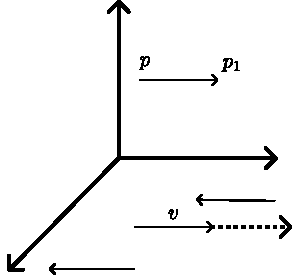
\includegraphics[scale=0.5]{cm1.pdf}
	\caption{Construcción de vectores}
\end{figure}

\subsubsection{Proyección ortogonal de vectores}

\begin{figure}[h!]
	\centering
	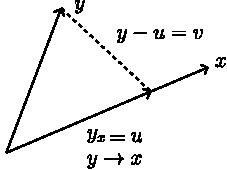
\includegraphics[width=0.4\textwidth]{cm2.pdf}
	\caption{Proyección}
\end{figure}

\begin{align*}
	 & u=\lambda x \text{ al mismo tiempo se tiene que cumplir:}                                                \\
	 & v\dot x=0 \text{ Condición de ortogonalidad}                                                             \\
	 & \implies (y-u)x=0\implies (y-\lambda x)x=0                                                               \\
	 & y\cdot x-\lambda x\cdot x=0\implies \lambda (x\cdot x)=y\cdot x                                          \\
	 & \therefore \lambda=\frac{y\cdot x}{x\dot x}\implies \lambda=\frac{y\cdot x}{\left\lVert x\right\rVert^2}
\end{align*}

Finalmente la Proyección en $Y_x=$

\begin{equation}
	Y_x=\frac{y\cdot x}{\left\lVert x\right\rVert^2}\cdot x
\end{equation}

Usando el resultado anterior:

\begin{align*}
	 & \cos \theta=\frac{\left\lVert \frac{y\cdot x}{\left\lVert x\right\rVert^2} \cdot x\right\rVert}{\left\lVert Y\right\rVert}=\frac{\left\lVert \frac{y\cdot x}{\left\lVert x\right\rVert}\cdot \frac{x}{\left\lVert x\right\rVert}\right\rVert^2}{\left\lVert y\right\rVert} \\
	 & \cos \theta=\frac{\left\lvert y\cdot x\right\rvert }{\left\lVert y\right\rVert\cdot \left\lVert x\right\rVert}
\end{align*}

\begin{definition}[Producto Vectorial]
	Sean $x,y \in \R^3$  denotado por $x\times y$ como:
	\begin{equation}
		x\times y=\det\begin{bmatrix}
			\hat{i} & \hat{j} & \hat{k} \\
			x_1     & x_2     & x_3     \\
			y_1     & y_2     & y_3
		\end{bmatrix}
	\end{equation}
	\begin{align}
		 & x\times y=\left( x_2y_3-y_2x_3-x_1y_3+y_1x_3,x_1y_2-y_1x_2 \right) \\
		 & x:\R^3\to \R^3
	\end{align}
\end{definition}

\subsubsection{Propiedades del producto vectorial}

Sean $x,y,z\in \R^3\land \lambda \in \R$ entonces
\begin{align}
	 & \text{Propiedades de ortogonalidad }(x\times y)\cdot x=0                                                                                                                \\
	 & \text{Propiedades de ortogonalidad }(x\times y)\cdot y=0                                                                                                                \\
	 & \text{Propiedades de no conmutatividad }x\times y=-y\times x                                                                                                            \\
	 & x\times (y+\lambda z)=(x\times y)+(\lambda x\times z)                                                                                                                   \\
	 & (x+\lambda y)\times z=(x\times z)+(\lambda y\times z)                                                                                                                   \\
	 & x\times y=0\longleftrightarrow x,y \text{ Son linealmente dependientes}                                                                                                 \\
	 & \left\lVert x\times y\right\rVert=\left\lVert x\right\rVert\left\lVert y\right\rVert \left\lvert \sin \theta \right\rvert  \text{Donde $\theta$ es el ángulo entre }x,y
\end{align}

\begin{exercise}[Propiedades de ortogonalidad $(x\times y)\cdot x=0$]
	\begin{align*}
		 & =\left( x_2y_3-y_2x_3,-x_1y_3+y_1x_3,x_1y_2-y_1x_2  \right)\left(x_1,x_2,x_3\right) \\
		 & =x_2y_3x_1-y_2x_3x_1-x_1y_3x_2+y_1x_3x_2+x_1y_2x_3-y_1x_2x_3                        \\
		 & =0
	\end{align*}
\end{exercise}


\begin{figure}[h!]
	\centering
	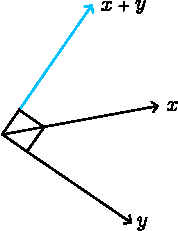
\includegraphics[width=0.2\textwidth]{cm3.pdf}
	\caption{Demostración geométrica}
\end{figure}

\begin{exercise}[Si $x,y\in \R^3\implies x\times y=-y\times x$]
	\begin{align*}
		 & x\times y= \begin{bmatrix}
			              \hat{i} & \hat{j} & \hat{k} \\
			              x_1     & x_2     & x_3     \\
			              y_1     & y_2     & y_3
		              \end{bmatrix}=-1\det\begin{bmatrix}
			                                  \hat{i} & \hat{j} & \hat{k} \\
			                                  x_1     & x_2     & x_3     \\
			                                  y_1     & y_2     & y_3
		                                  \end{bmatrix} \\
		 & =-y\times x
	\end{align*}
\end{exercise}

\begin{exercise}[$x\times y=0\longleftrightarrow x,y$ Son linealmente dependientes]
	Implica que $x,y$ son linealmente dependientes, por lo que $x=\lambda y$ ó $y=\lambda x$
	entonces $x\times y=x\times (\lambda x)$
	\begin{align*}
		 & =\det\begin{bmatrix}
			        \hat{i} & \hat{j} & \hat{k} \\
			        x_1     & x_2     & x_3     \\
			        y_1     & y_2     & y_3
		        \end{bmatrix}                                                                                                                                                   \\
		 & =\hat{i}\left(x_2\cdot \lambda x_3-\lambda x_2 x_3 \right)-\hat{j}\left(x_1\cdot \lambda x_3 -\lambda x_1 x_3\right)+\hat{k}\left(x_1\cdot \lambda x_2-\lambda x_1\cdot x_2\right) \\
		 & =\lambda \hat{i}(0)-\lambda \hat{j}(0)+\lambda\hat{k}(0)=                                                                                                                          \\
		 & =(0,0,0)=\bar{0}
	\end{align*}
\end{exercise}



\begin{exercise}[Si $x,y \in \R^3\implies \left\lVert x\times y\right\rVert=\left\lVert x\right\rVert\left\lVert y\right\rVert \left\lvert \sin \theta \right\rvert $]
	\begin{align*}
		 & \left\lVert x\times y\right\rVert^2=\left(x_2y_3-x_3y_2\right)^2+\left(-x_1y_3+x_3y_1\right)^2+\left(x_1y_2-y_1x_2\right)^2                                                                                                                                                                                    \\
		 & =x_2^2y_3^2-2x_1y_3x_3y_2+x_3^2y_2^2+x_1^2y_3^2-2x_1y_3x_3y_1+x_3^2y_1^2+x_1^2y_2^2-2x_1y_2y_1x_2+y_1^2x_2^2                                                                                                                                                                                                   \\
		 & =x_z^2y_1^2-x_1^2y_1^2+x_1^2y_2^2+x_1^2y_3^2+x_2^2y_1^2+x_2^2y_2^2-x_2^2y_2^2+x_2^2y_3^2+x_3^2y_1^2+x_3^2y_2^2+x_3^2y_3^2-x_3^2y_3^2\dots                                                                                                                                                                      \\
		 & \dots 2x_1x_2y_1y_2-2x_1x_3y_1y_3-2x_2x_3y_2y_3=x_1^2\left( y_1^2+y_2^2+y_3^2\right)+x_2^2\left(y_1^2+y_2^2+y_3^2\right)\dots                                                                                                                                                                                  \\
		 & \dots+x_3^2\left(y_1^2y_2^2+y_3^2\right)-\left(x_2^2y_1^2+x_2^2y^2+x_2^2y_3^2+2x_2x_2y_1y_2+ 2x_1x_3y_1y_3+2x_2x_3y_2y_3\right)                                                                                                                                                                                \\
		 & =\left(x_1^2+x_2+x_3^2\right)\left(y_1+y_2+y_3\right)-\left(x_1y_1+x_2y_2+x_3y_3\right)^2                                                                                                                                                                                                                      \\
		 & =\left\lVert x\right\rVert^2\cdot \left\lVert y\right\rVert -\left(x\cdot y\right)^2=\left\lVert x\right\rVert \cdot \left\lVert y\right\rVert -\left\lVert x\right\rVert^2\cdot \left\lVert y\right\rVert^2\cos^2\theta=\left\lVert x\right\rVert^2\cdot \left\lVert y\right\rVert^2\left(1-\cos\theta\right) \\
		 & \left\lVert x\times y\right\rVert=\left\lVert x\right\rVert^2 \cdot \left\lVert y\right\rVert^2\sin{\theta}\implies \left\lVert x\times y\right\rVert=\left\lVert x\right\rVert \cdot \left\lVert y\right\rVert \left\lvert \sin{\theta} \right\rvert
	\end{align*}
\end{exercise}

\subsection{El triple producto escalar}

Sean $x,y,z\in \R^3$, entonces el triple producto escalar será:

\begin{equation}
	x\cdot\left(y\times z\right)= \det\begin{bmatrix}
		x_1 & x_2 & x_3 \\y_1&y_2&y_3\\ z_1&z_2&z_3
	\end{bmatrix}
\end{equation}

\begin{proof}[El desarrollo del producto vectorial $y\times z$]
	\begin{align*}
		y\times z=\det\begin{bmatrix}
			              \hat{i} & \hat{j} & \hat{k} \\y_1&y_2&y_3\\ z_1&z_2&z_3
		              \end{bmatrix}=\hat{i}(y_2z_3-z_2y_3)-\hat{j}(y_1z_3-z_1y_3)+\hat{k}(y_1z_2-z_1y_2) \\
		y\times z=\left(y_2z_3-z_2y_3,-y_1z_3+z_1y_3,y_1z_2-z_1y_2\right)
	\end{align*}

	Luego el triple producto será:
	\begin{align*}
		 & x\cdot(y\times z)=(x_1,x_2,x_3)\cdot(y_2z_3-z_2y_3,-y_1z_3+z_1y_3,y_1z_2-z_1y_2) \\
		 & =x_1(y_2z_2-z_2y_3)-x_2(y_1z_3-z_1y_2)+x_3(y_1z_2-z_1y_2)                        \\
		 & =x_1\det\begin{bmatrix}
			           y_2 & y_3 \\z_2&z_3
		           \end{bmatrix}-x_2\det\begin{bmatrix}
			                                y_1 & y_3 \\z_1&z_3
		                                \end{bmatrix}+x_3\det\begin{bmatrix}
			                                                     y_1 & y_2 \\z_1&z_2
		                                                     \end{bmatrix}             \\
		 & \therefore x\cdot (y\times z)=\det\begin{bmatrix}
			                                     x_1 & x_2 & x_3 \\y_1&y_2&y_3\\ z_1&z_2&z_3
		                                     \end{bmatrix}
	\end{align*}
\end{proof}

Si $x,y\in \R^3\implies \left\lVert x\times y\right\rVert=$ área del paralelogramo formada por los vectores $x$ y $y$


\begin{figure}[h!]
	\centering
	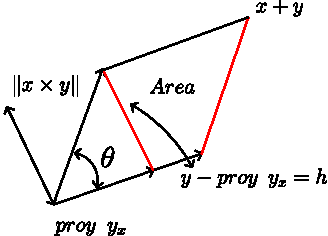
\includegraphics[width=0.4\textwidth]{cm4.pdf}
	\caption{Proyecciones en el Paralelogramo}
\end{figure}

\begin{align*}
	 & A=B\times h                                                                                        \\
	 & A=\left\lVert x\right\rVert\left(y-Proy\quad Y_x\right)                                            \\
	 & A=\left\lVert x\right\rVert\left\lVert y\right\rVert\sin{\theta}=\left\lVert x\times y\right\rVert
\end{align*}


Sean $x,y,z\in \R^3$, el volumen del paralelepípedo formado por los vectores $x,y,z$ es:

\begin{equation}
	V=\left\lvert x\cdot(y\times z)\right\rvert
\end{equation}

\begin{figure}[h!]
	\centering
	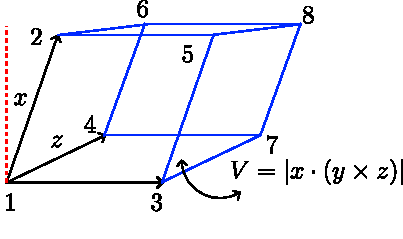
\includegraphics[width=0.6\textwidth]{cm5.pdf}
	\caption{Proyecciones en el Paralelepípedo}
\end{figure}


El área de la base del paralelepípedo
es igual a $\left\lVert x\times y\right\rVert$,
en tanto que la altura se podría calcular como la
norma de la proyección del vector $x$ sobre un vector
perpendicular $y$ y a $z$, ese vector puede ser $y\times z$:

\begin{equation*}
	Proy\quad X_{y\times z}=\frac{x\cdot(y\times z)}{\left\lVert x\times y\right\rVert}\cdot (y\times z)
\end{equation*}

Por lo tanto la altura del paralelepípedo será $Proy\quad X_{y\times z}$:

\begin{align*}
	 & h=Proy\quad X_{y\times z}=\left\lVert \frac{x\cdot(y\times z)}{\left\lVert x\times y\right\rVert^2}\cdot (y\times z) \right\rVert                                                                               \\
	 & h=\left\lvert \frac{x\cdot (y\times z)}{\left\lVert x\times y\right\rVert^2}\right\rvert \left\lVert x\times y\right\rVert=\frac{\left\lvert x\cdot (y\times z)\right\rVert}{\left\lVert x\times y\right\rVert}
\end{align*}

Finalmente el volumen será Área de la base por altura:

\begin{equation*}
	V=\left\lVert x\cdot (y\times z)\right\rVert
\end{equation*}


\section{Rectas y planos en R3}

\begin{definition}[Rectas]
	Para determinar una recta en el espacio de $\R^3$ es suficiente conocer:
	\begin{enumerate}
		\item Un punto por donde pasa
		\item Un vector de dirección. (El cual puede estar o no contenido en la recta en cuyo caso sería un vector paralelo)
	\end{enumerate}
\end{definition}

Si $\overrightarrow{V}=(V_z,V_2V_3)$ es un vector de dirección de la recta $l$ y la recta pasa por el punto $P=(x_1,x_2,x_3)$, entonces cualquier punto $q=(q_1,q_2,q_3)$
pertenecerá a $l$ sí y sólo sí el vector $q-p=(q_1-x_1,q_2-x_2,q_3-x_3)$ es paralelo al vector $V$, es decir:

\begin{align*}
	 & q_1-x_1=tv_1 &  & q_1=x_1+tv_1 \\
	 & q_2-x_2=tv_2 &  & q_2=x_2+tv_2 \\
	 & q_3-x_3=tv_3 &  & q_3=x_3+tv_3
\end{align*}

Donde $t\in \R$ al conjunto se le conoce como ecuaciones paramétricas de la recta $l$.

Si se manipulan las ecuaciones del conjunto, se obtienen otras formas de expresar la ecuación de una recta:

Si se despeja cada ecuación el parámetro $t$ se tiene:

\begin{align*}
	 & t=\frac{q_1-x_1}{v_1} &  & t=\frac{q_2-x_2}{v_2} &  & t=\frac{q_3-x_3}{v_3}
\end{align*}

igualándolas y considerando que $V$ el vector de dirección es un vector no nulo:

\begin{align*}
	 & \frac{q_1-x_1}{v_1}=\frac{q_2-x_2}{v_2}=\frac{q_3-x_3}{v_3}         \\
	 & \text{Se le conocen como ecuaciones simétricas de la recta en }\R^3
\end{align*}

Considerando nuevamente el conjunto de ecuaciones paramétricas de la recta:

\begin{align*}
	 & q_1-x_1=tv_1 &  & l(t)=(x_1,x_2,x_3)+t(v_1,v_2,v_3)     \\
	 & q_2-x_2=tv_2 &  & \implies l(t)=x+t\overrightarrow{V}   \\
	 & q_3-x_3=tv_3 &  & \text{Ecuación vectorial de la recta}
\end{align*}


\begin{equation}
	Ax+By+Cz+D=0 \text{ Ecuación general del plano}
\end{equation}

Los coeficientes $A,B$ y $C$ son las coordenadas del vector ortogonal (normal) del plano.


\begin{example}
	Determina la ecuación del plano que pasa por el punto (2,1,3) y tiene como vector normal al vector $\overrightarrow{N}=\left(2,-4,5\right)$
\end{example}

\textit{ Sol. }

\begin{align*}
	 & 2(x-2)+(-4)(y-1)+5(z-3)=0 \\
	 & 2x-4-4y+4+5z-15=0         \\
	 & 2x-4y+5z-15=0
\end{align*}

Para graficar, se calculan las intersecciones:

\begin{align*}
	 & 2x-4y+5z=15\implies \frac{2x}{15}'\frac{4y}{15}+\frac{5z}{15}=1 \implies \frac{x}{\frac{15}{2}}+\frac{y}{\frac{-15}{4}}+\frac{z}{3}=1
\end{align*}


\begin{example}
	Determine si los puntos p=(0,0,1) y q=(1,1,-1) pertenecen al plano $\pi=3x-y+z=1$
\end{example}

\textit{ Sol. }

\begin{align*}
	 & 3(0)-(0)+(1)=0-0+1=1=1  \\
	 & \therefore p\in \pi     \\
	 & 3(1)-(1)+(-1)=3-1-1=1=1 \\
	 & \therefore q\in \pi
\end{align*}

\begin{example}
	Calcula la ecuación de la recta de los puntos $q=(2,1,5)$ y $r=(8,4,2)$
\end{example}

\textit{ Sol. }

\begin{align*}
	 & \overrightarrow{qp}=\overrightarrow{qr}=(2,1,5)-(8,4,2)=(-6,-3,-2)                                                                                   \\
	 & \overrightarrow{N}=\overrightarrow{qp}\times \overrightarrow{qr}=\det \begin{bmatrix}
		                                                                         \hat{i} & \hat{j} & \hat{k} \\
		                                                                         -7      & -5      & -3      \\
		                                                                         -6      & -3      & -2
	                                                                         \end{bmatrix}=\overrightarrow{N}=\hat{i}(-15-9)-\hat{j}(-21-18)+\hat{k}(21-30)
\end{align*}

\begin{definition}
	Sea $A\in M_{n\times n}(\R)$ si $n=1$ entonces $A=A_{11}$
	en este caso el $\det(A)=A_{11}$. Para $n\geq 2$ se define el determinante de $A$ como:
	\begin{align}
		 & \det(A)=\sum_{j=1}^n(-1)^{1+j}A_{ij}\cdot \det\left(\bar{A}_{1j}\right)                                                                                      \\
		 & A=\begin{bmatrix} a_{11}&a_{12}&a_{13}\\ a_{21}&a_{22}&a_{23}\\ a_{31}&a_{32}&a_{33}\\ \end{bmatrix}\implies \text{Formula de Laplace}                       \\
		 & det(A)=\sum_{j=1}^3(-1)^{1+j}a_{1j}\cdot det(\bar{A}_{1j})                                                                                                   \\
		 & =(-1)^{1+1}a_{11}\det(\bar{A}_{11})+(-1)^{1+2}\cdot \det(\bar{A}_{12})+(-1)^{1+2}a_{13} \det(\bar{A}_{13})                                                   \\
		 & =(-1)^2a_{11}\cdot\det\begin{bmatrix} a_{21}&a_{23}\\ a_{31}&a_{33}\end{bmatrix}+(-1)^4a_{13}\det\begin{bmatrix} a_{21}&a_{22}\\ a_{31}&a_{33} \end{bmatrix}
	\end{align}
\end{definition}


Al vector obtenido se le llamará vector normal del plano

\begin{equation*}
	\overrightarrow{N}=-24\hat{i}+39\hat{j}-9\hat{k}
\end{equation*}

Se aplica la expresión $\overrightarrow{N}\cdot \left(\overrightarrow{x-x_0}\right)=0$

\begin{align*}
	 & (-24,39,-9)\cdot (x-8,1-4,z-2)=0                             \\
	 & -24x+192+39y-156-9z+18=0                                     \\
	 & -24x+39y-9z+54=0                                             \\
	 & \text{Ecuación del plano que pasa por los tres puntos dados}
\end{align*}

Ahora se comprobará que los tres puntos están en el plano.
Para el punto $P=(1,-1,-1)$:
\begin{align*}
	 & -24(1)+39(-1)-9(-1)+54= \\
	 & -24-39+9+54=            \\
	 & 54-54=0
\end{align*}

El punto $q\in \pi$

\begin{example}
	Demuestre que los planos: $x+y+z=6$, $x-y-z=0$, $2x-3y+z=1$ se cortan en un solo punto. Determine este punto:
\end{example}

\textit{ Sol. }

Se verificará el determinante asociado al sistema de ecuaciones definido por los tres planos llamado $\sigma$:

\begin{equation*}
	\begin{cases}
		 & x+y+z  =6 \\
		 & x-y-z  =0 \\
		 & 2x-3y+z=1
	\end{cases}\implies\det\left(\sigma\right)=\det\begin{bmatrix}
		1 & 1 & 1 \\1&-1&-1\\2&-3&1
	\end{bmatrix}
\end{equation*}

Como el Determinante es distinto de cero, el sistema de ecuaciones tiene una solución única.
Si los resolvemos con el método de Gauss-Jordan, obtenemos que $x=1$, $y=2$ y $z=1$
Por lo tanto el punto de intersección de los tres puntos en el plano es: $P=(3,2,1)$

\begin{example}
	Determine la recta de intersección de los planos
	$\pi_1:x+y+5z-1=0$ y $\pi_2=2x+3y-z+2=0$
\end{example}

\textit{ Sol. }

La intersección de los planos se determinará resolviendo el sistema de ecuaciones:

\begin{equation*}
	\begin{cases}
		 & x+y+5z-1=0 \\
		 & 2x+3y-z2=0
	\end{cases}.
\end{equation*}

La matriz asociada al sistema de ecuaciones.

\begin{equation*}
	\begin{bmatrix}
		1 & 1 & 5  & -1 \\
		2 & 3 & -1 & -2 \\
	\end{bmatrix}\implies  \begin{bmatrix}
		1 & 0 & 16  & 5  \\
		0 & 1 & -11 & -4 \\
	\end{bmatrix}
\end{equation*}

El sistema de ecuaciones equivalentes al sistema de ecuaciones original es:

\begin{equation*}
	\begin{cases}
		 & x=5-16t  \\
		 & y=-4+11t \\
		 & z=t
	\end{cases}.
\end{equation*}

Las ecuaciones paramétricas de la recta de intersección de los planos $\pi_1$ y $\pi_2$

Que en forma vectorial sería:

\begin{align*}
	 & l(t)=\left(x(t),y(t),z(t)\right)=(5,-4,0)+(-16,11,1)                     \\
	 & \implies l(t)=(5,-4,0)+t(-16,11,1)                                       \\
	 & X_0=(5,-4,0)\text{ Es un punto por donde pasa } l(t)                     \\
	 & \overrightarrow{V}=(-16,11,1) \text{ Es el vector de dirección de } l(t)
\end{align*}

\begin{example}
	Hallar la ecuación del plano que pasa por los puntos $A=(2,-1,4)$ y $B=(3,2,-1)$
	y que es perpendicular al plano $\pi: x+y+2z=0$
\end{example}

\textit{ Sol. }

\begin{equation*}
	\overrightarrow{N}\cdot \overrightarrow{n}=0\land \overrightarrow{N}\cdot \overrightarrow{AB}=0\implies \overrightarrow{N}=\overrightarrow{n}\cdot \overrightarrow{AB}
\end{equation*}

Al hacer los cálculos:
\begin{align*}
	 & \overrightarrow{N}=\det\begin{bmatrix}
		                          \hat{i} & \hat{j} & \hat{k} \\
		                          1       & 1       & 2       \\ 1&3&-5
	                          \end{bmatrix}\implies \overrightarrow{N}=\hat{i}(-5-6)-\hat{j}(-5-2)+\hat{k}(3-1) \\
	 & \overrightarrow{N}=-11\hat{i}+7\hat{j}+2\hat{k}\text{ Es el vector normal del plano}
\end{align*}
Ahora se aplica la ecuación vectorial del plano

\begin{align*}
	 & \overrightarrow{N}\cdot (\overrightarrow{x-x_0})=0                \\
	 & (-11,7,2)\cdot (x-2,y+1,z-4)=0\implies-11x+22+7y+7+2z-8=0\implies \\
	 & -11x+7y+2z+21=0\text{ Es la ecuación del plano}
\end{align*}

Ahora se comprobará que el plano encontrado satisface las dos condiciones (las cuales se usaron para su construcción)

\begin{enumerate}
	\item Debe contener a los puntos $A$ y $B$ para el punto $A=(2,-1,4)$ $-11(2)+7(-1)+2(4)+21=-22-7+8+21$ y es igual a $0,\therefore A\in \pi_1$
	      Para el punto $B=(3,2,-1)$, $-11(3)+7(2)+2(-1)+21=-33+14-2+21$ es igual a 0, $\therefore B\in \pi_1$

	\item El plano encontrado deberá ser perpendicular al plano dado, es decir que los vectores normales de los planos deben ser ortogonales $(\overrightarrow{N}\cdot \overrightarrow{n}=0)$
	      \begin{align*}
		       & \overrightarrow{N}=(-11,7,2); \overrightarrow{n}=(1,1,2)                   \\
		       & \overrightarrow{N}\cdot \overrightarrow{n}=(-11,7,2)\cdot(1,1,2)=-11+7+4=0
	      \end{align*}
	      Como los vectores normales de los planos son ortogonales, los planos también lo son.
\end{enumerate}

\section{Funciones de una variable}
\begin{align*}
	 & \text{Funciones del tipo}                &  & \text{Funciones del tipo}            \\
	 & f:\R\to \R^n                             &  & f:\R^n\to \R                         \\
	 & \text{Funciones con valores vectoriales} &  & \text{Funciones de varias variables}
\end{align*}

El gráfico asociado con una función del tipo $f:\R\to \R^n$ es una curva.
Mientras que el gráfico asociado con una función del tipo $f:\R^n\to \R$ es una superficie.

\begin{definition}[Trayectoria en $\R^n$]
	Es una función $\sigma:\left[a,b\right]\to \R^n$. Si $\sigma$ es diferenciable, decimos que $\sigma$
	Es una trayectoria diferenciable. Si $\sigma$ es de clase $C^1$, decimos que $\sigma$ es una $C^1-trayectoria$.
	Los puntos $\sigma(a)$ y $\sigma(b)$, se llaman extremos de la trayectoria; la imagen de $\sigma$ se le llama curva de $\sigma$.
\end{definition}

\begin{example}
	La recta $l(t)$ en $\R^3$ que pasa por el punto $x_0=(x_0,y_0,z_0)$ en la dirección del vector $\overrightarrow{V}$ es la curva de la trayectoria
	\begin{equation*}
		\sigma(t)=x_0+t\overrightarrow{V}; t\in \R
	\end{equation*}
	Si $x_0=(1,2,3)$ y $\overrightarrow{V}=(5,-1,2)$ implica que al evaluar:
	\begin{align*}
		 & \sigma(0)=(1,2,3)+t(5,-1,2)= \\
		 & \sigma(0)=(1,2,3)+0(5,-1,2)= \\
		 & \sigma(0)=(1,2,3)\in \R^3    \\
		 & \sigma(1)=(1,2,3)+1(5,-1,2)= \\
		 & \sigma(1)=(1,2,3)+(5,-1,2)=  \\
		 & \sigma(1)=(6,1,5)\in \R^3
	\end{align*}
\end{example}


\begin{example}
	Considérese la ecuación $x^2+y^2=1$ la cual representa en $\R^2$ un círculo unitario.

	Para la ecuación $x^2+y^2=1$ como una trayectoria, se propondrá un cambio de variables en coordenadas polares
	\begin{align*}
		 & x=r\cos\theta &  & y=r\sin{\theta}
	\end{align*}
	Como el círculo es unitario, el radio es uno.
	\begin{align*}
		\sigma:\R\to \R^2;\sigma(\theta)\left(\cos\theta,\sin{\theta}\right) \\
		\sigma=\left[0,2\pi\right]\to \R^2\footnote{La imagen de $\sigma(\theta)$ es el círculo unitario}
	\end{align*}
	Continuando con el cambio de coordenadas:
	\begin{align*}
		 & x(r,0)=r\cos(\theta);y(r,\theta)=r\sin(\theta)                                                                                   \\
		 & x^2+y^2=r^2\cos^2(\theta)+r^2\sin^2(\theta)\implies                                                                              \\
		 & x^2+y^2=r^2\left(\cos^2\theta+\sin^2\theta\right)\implies                                                                        \\
		 & x^2+y^2=r^2\implies \frac{y}{x}=\frac{r\sin\theta}{r\cos\theta}=\frac{\sin{\theta}}{\cos\theta}\begin{cases}
			                                                                                                  x\neq 0 \\
			                                                                                                  x\neq \frac{\pi}{2},\frac{3\pi}{2}
		                                                                                                  \end{cases} \\
		 & \frac{y}{x}=\tan\theta\implies \theta=\arctan\left(\frac{y}{x}\right)
	\end{align*}
\end{example}


\begin{example}
	Determine una parametrización para la parábola $y(x)=x^2$

	\textit{ Sol. }

	Sea $r(t)=(t,t^2); t\in \left[0,1\right]$
\end{example}

\begin{example}
	Obtenga la ecuación en coordenadas polares de la ecuación cartesiana $\left(x^2+y^2\right)^2=8xy$
\end{example}

\textit{ Sol. }

Se sabe que $x=r\cos\theta,y=\sin{\theta}$

\begin{align*}
	 & x^2+y^2=r^2                 \\
	 & \theta=\arctan{\frac{4}{x}}
\end{align*}

Sustituyendo lo anterior en la ecuación cartesiana:

\begin{align*}
	 & \left(r^2\right)^2=8\left(r\cos{\theta}\right)\left(r\sin{\theta}\right)\mid r\neq 0 \\
	 & r^2=4\sin{2\theta}
\end{align*}


\begin{example}
	¿Qué representa en coordenadas cartesianas la ecuación polar $r=2\cos{2\theta}$?

\end{example}

\textit{ Sol. }

Sustituyendo por lo conocido del cambio de coordenadas:

\begin{align*}
	 & \sqrt{x^2+y^2}=\frac{2x}{\sqrt{x^2+y^2}}\implies x^2+y^2=2x \\
	 & x^2-2x+1+y^2=0\implies (x-1)^2+(y-0)^2=1                    \\
	 & \text{Es una circunferencia de radio 1 y centro (1,0)}
\end{align*}

\begin{example}
	¿Qué representa en coordenadas cartesianas la ecuación $r=4\sin{\theta}$?
\end{example}

\begin{align*}
	 & \sqrt{x^2+y^2}=\frac{4y}{\sqrt{x^2+y^2}}\implies x^2+y^2=4y \\
	 & x^2+y^2-4y+4=0                                              \\
	 & (x-0)^2+(y-2)^2=4                                           \\
	 & \text{Es una circunferencia de radio 2 y centro (0,2)}
\end{align*}

\subsubsection{Gráficas en coordenadas polares}


\begin{figure}[h!]
	\centering
	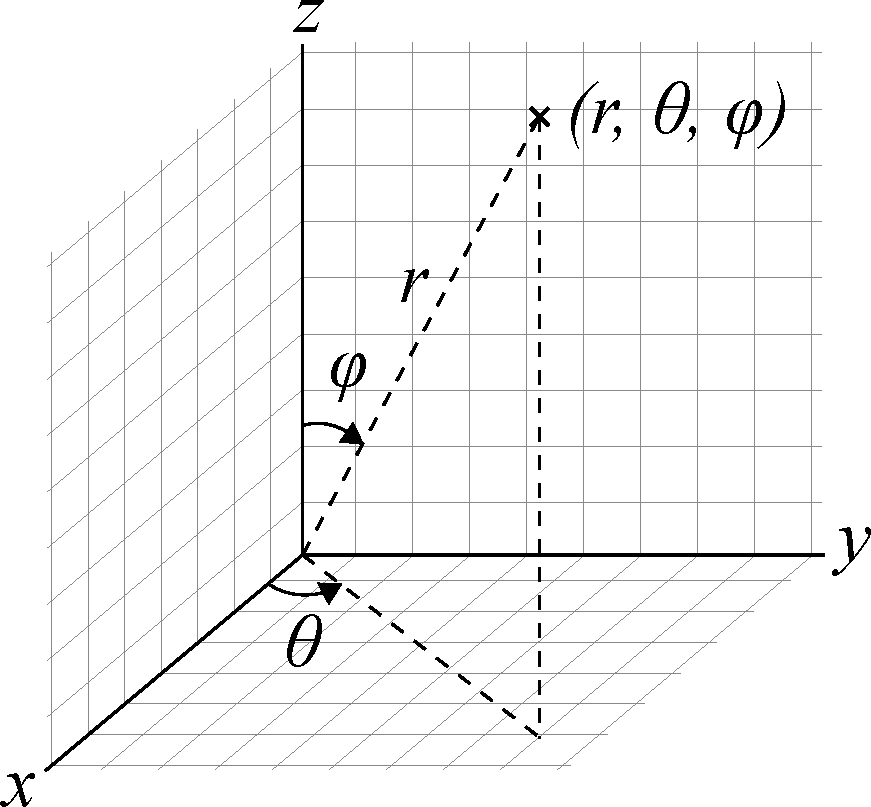
\includegraphics[width=0.6\textwidth]{cm6.pdf}
	\caption{Representación de una coordenada polar}
\end{figure}

Considere la siguiente ecuación:

$r=\cos{2\theta}$ que tiene por gráfica (figura \ref{cm6}) en coordenadas cartesianas ángulo vs radio,
en tanto que en coordenadas polares es:


\begin{figure}[h!]
	\centerline{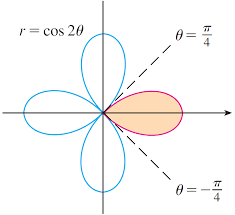
\includegraphics[width=0.3\textwidth]{cm6.png}}
	\caption{Función en coordenadas polares}
	\label{cm6}
\end{figure}



Si ya se conoce un vector tangente a la curva $\sigma(t)\forall t\in \left[a,b\right]$
es posible calcular una recta tangente a $\sigma(t)$ en $t_0\in\left[a,b\right]$
la cual tendría la forma:

\begin{equation*}
	l(t))\left(x_0,y_0,z_0\right)+t\overrightarrow{v}
\end{equation*}

$\overrightarrow{v}$ el vector de dirección será el vector tangente a $\sigma(t)$
en $t_0$ $\sigma(t_0)=\left(\sigma_1(t_0),\sigma_2(t_0),\sigma_3(t_0)\right)$
y $\overrightarrow{v}=\sigma^{\prime}(t_0)=\left(\sigma^{\prime}_1(t_0),\sigma^{\prime}_2(t_0),\sigma^{\prime}_3(t_0)\right)$

Así la recta tangente a $\sigma$ en $\sigma(t_0)$ será:

\begin{equation}
	l\left(\sigma(t_0)\right)=\left(\sigma_1(t_0),\sigma_2(t_0),\sigma_3(t_0)\right)+t\sigma^{\prime}_1(t_0),\sigma^{\prime}_2(t_0),\sigma^{\prime}_3(t_0)
\end{equation}

Con $t\in \R$

\begin{definition}[Rapidez]
	Sea $\sigma(t)$ una función $\sigma:\left[a,b\right]\to \R$ de
	clase $C^1$ se define la velocidad $\sigma^{\prime}(t)$ el vector
	$\sigma^{\prime}(t)=\left(\sigma_1^{\prime}(t),\sigma_2^{\prime}(t),\dots ,\sigma_{n}^{\prime}(t)\right)$
	En tanto que la rapidez se definirá como $X\left\lVert \sigma^{\prime}(t)\right\rVert$

	\begin{equation}
		\left\lVert \sigma^{\prime}(t)\right\rVert=\sqrt{\left(\sigma_1^{\prime}(t)\right)^2,\left(\sigma_2^{\prime}(t)\right)^2,\dots ,\left(\sigma_{n}^{\prime}(t)\right)^2}
	\end{equation}

\end{definition}


\begin{problem}
Si $\sigma(t)=\left(\cos{(t)},\sin{(t)},t\right)$ determine:
\begin{enumerate}
	\item La recta tangente en el punto (1,0,0)
	\item El vector velocidad
	\item La rapidez en cualquier punto de $\sigma(t)$
\end{enumerate}
\end{problem}

\textit{ Sol. }

Se verifica que el punto dado pertenezca a la cruz es decir:

\begin{align*}
	 & (1,0,0)=\left(\cos{(t)},\sin{t},t\right)\implies \\
	 & 1=\cos{(t)},\land 0=\sin{t},\land 0=t            \\
	 & \text{Como t es cero, al sustituir}              \\
	 & \cos{(0)}=1\land \sin{(0)}=0                     \\
	 & \therefore P_0=(1,0,0)\in\sigma
\end{align*}

El punto de tangencia es correcto, ahora se calcula el vector tangente a la curva
$\sigma$ en $P_0$, es decir:

\begin{align*}
	 & \sigma(t)=\left(\cos{(t)},\sin{t},t\right)                              \\
	 & \sigma^{\prime}(t)=\left(-\sin{t},\cos{(t)},1\right)=                   \\
	 & \text{Vector velocidad en todo punto del dominio} \sigma \forall t\in I
\end{align*}

La velocidad en $P_0=(1,0,0)$ será
$sigma^{\prime}(t=0)=\left(-\sin{t},\cos{(t)},1\right)$
$sigma^{\prime}(0)=(0,1,1)=\overrightarrow{V}$ el vector de dirección de la recta tangente.

Por lo tanto la recta tangente a $\sigma$ en el punto es:

\begin{align*}
	 & l(t)=\sigma(P_0)+ t\sigma^{\prime}(P_0)                                                   \\
	 & l(t)=(1,0,0)+t(0,1,1)\implies l(t)=(1,t,t)                                                \\
	 & l(t)=V=\left(-sin{(t)},\cos(t),1\right)                                                   \\
	 & \left\lVert V\right\rVert=\sqrt{\left(-\sin^2{(t)}\right)^2+\left(\cos{(t)}\right)^2+1^2} \\
	 & \left\lVert V\right\rVert=\sqrt{\sin^2{(t)}+\cos^2{(t)} +1}                               \\
	 & \left\lVert V\right\rVert=\sqrt{2}
\end{align*}

\begin{align*}
	 & \sigma(t)=\left(\cos{(t)},\sin{t},t\right) \\
	 & \sigma(\pi)=(-1,0,\pi)                     \\
	 & \sigma:\left[a,b\right]\to \R^3
\end{align*}

\begin{definition}
	Sea $\sigma:\left[a,b\right]\to\R^n$ Una trayectoria de clase $C^1$. La longitud de
	$\sigma$ para determinado intervalo contenido en $\left[a,b\right]$ está dada por:
	\begin{equation}
		L\left(\sigma\right)=\int \left\lVert \sigma^{\prime}(t)\right\rVert\,dt
	\end{equation}
	Para el caso en el que $n=3\left(\sigma:\left[a,b\right]\to \mathbb{3}^3\right)$ la fórmula se ve como:
	\begin{equation*}
		L\left(\sigma\right)=\int_{a_0}^{a_1}\sqrt{\left(\sigma_1^{\prime}(t)\right)^2+\left(\sigma_2^{\prime}(t)\right)^2+\left(\sigma_3^{\prime}(t)\right)^2}\, dt\\
		\text{Donde} [_0.a_1]\subset \left[a,b\right]
	\end{equation*}
\end{definition}


\begin{problem}
Determine la longitud de arco de la curva
\begin{equation*}
	\sigma(t)=\left(r\cos{(t)}\right)
\end{equation*}
\end{problem}


\textit{ Sol. }

\begin{align*}
	 & L\left(\sigma\right)=\int_{0}^{2\pi}\sqrt{\left(-r\sin{(t)}\right)^2+\left(r\cos{(t)}\right)^2}\, dt \\
	 & L\left(\sigma\right)=\int_{0}^{2\pi} \sqrt{r^2}\, dt                                                 \\
	 & L\left(\sigma\right)=\int_{0}^{2\pi} r\, dt=r\cdot t=r(2\pi -0)                                      \\
	 & L\left(\sigma\right)=2\pi r
\end{align*}

%%%%%%%%%%%% GRAFICAAAAAAAAAAAAAAAAAAAAAAAAAAAAAAAAAAAAA

\begin{problem}
Sea $\sigma$ la trayectoria $\sigma(t)=\left(t,t\sin{(t)},t\cos{(t)}\right)$
Hallar la longitud de arco de $\sigma$ entre (0,0,0) y $(\pi,0,-\pi)$
\end{problem}

\textit{ Sol. }

Se debe cumplir lo siguiente\footnote{$\sigma:\left[a,b\right]\to \R^3\land t\to (x,y,z)$}:(Para $P_0=(0,0,0)$)

\begin{align*}
	 & (0,0,0)=\left(t,t\sin{(t)},t\cos{(t)}\right)\implies \\
	 & 0=t                                                  \\
	 & 0=t\sin{(t)}                                         \\
	 & 0=t\cos{(t)}
\end{align*}

Se sabe que $t=0$. se verificará que las ecuaciones son consistentes:
\begin{align*}
	 & 0\sin{0}=0\cdot 0=0 \\
	 & 0\cos{0}=0\cdot 1=0
\end{align*}

Se deberá cumplir lo siguiente para $P_1=(\pi,0,-\pi)$

\begin{align*}
	 & \pi=t           \\
	 & 0=t\sin{t}      \\
	 & -\pi=t\cos{(t)}
\end{align*}

Se tiene que $t=\pi$:

\begin{align*}
	 & \pi\cdot \sin{\pi}=\pi\cdot 0=0      \\
	 & \pi\cdot \cos{\pi}=\pi\cdot(-1)=-\pi
\end{align*}

Los límites para integrar el intervalo para el cual la longitud del arco es:

\begin{equation}
	l\left(\sigma (t)\right)=\int_a^b \left\lVert \sigma^{\prime}(t)\right\rVert\, dt
\end{equation}

De aquí obtenemos que:

\begin{align*}
	 & l\left(\sigma (t)\right)=\int_0^\pi \sqrt{1^2}\, dt
	 & \left\lVert \sigma^{\prime}(t)\right\rVert=\sqrt{\left(\sigma_1^{\prime}(t)\right)^2+\left(\sigma_2^{\prime}(t)\right)^2+\left(\sigma_3^{\prime}(t)\right)^2}
\end{align*}

\begin{align*}
	 & \sigma_1^{\prime}(t)=t &  & \sigma_2^{\prime}(t)=t\sin{(t)}         &  & \sigma_3^{\prime}(t)=t\cos{(t)}                \\
	 & \sigma_1^{\prime}(t)=1 &  & \sigma_2^{\prime}(t)=\sin{t}+t\cos{(t)} &  & \sigma_3^{\prime}(t)=\cos{(t)}-t\setminus{(t)}
\end{align*}


\begin{align*}
	 & l\left(\sigma (t)\right)=\int_0^\pi \sqrt{1+\sin^2{(t)}+2t\sin{(t)}\cos{(t)}+t^2\cos^2{t}+\cos^2{(t)}\dots}                             \\
	 & \sqrt{\dots -2t\cos{(t)}\sin{(t)}+t^2\sin^2{(t)}}=                                                                                      \\
	 & =l\left(\sigma (t)\right)=\int_0^\pi \sqrt{\sqrt{2+t2}}\, dt=\int_0^\pi \sqrt{t^2+(\sqrt{2})^2}\, dt=\frac{1}{2}\pi\sqrt{\pi^2+2}+\dots \\
	 & \ln{\left(\pi+\sqrt{\pi^2+2}\right)}-\ln{\left(0+\sqrt{0+2}\right)}=                                                                    \\
	 & l\left(\sigma (t)\right)=\frac{1}{2}\pi\sqrt{\pi^2+2}+\ln{\left(\pi+\sqrt{\pi^2+2}\right)-\ln{\left(\sqrt{2}\right)}}
\end{align*}

\begin{problem}
Se dice que una trayectoria $\sigma(S)$ está parametrizada por longitud de arco, o lo que es lo mismo, tiene rapidez unitaria si $\left\lVert \sigma^{\prime}(S)\right\rVert=1$
Muestre que para una trayectoria parametrizada por longitud de arco en $[a,b]$ se tiene que $l\left(\sigma(S)\right)=b-a$
\end{problem}

\textit{ Sol.}

\begin{proof}
	$\left[a,b\right]$ se tiene que $l\left(\sigma(S)\right)=b-a$

	Como $S=\sigma(t)$ entonces su derivada $\frac{dS}{st}=\sigma^{\prime}(t)$
	\begin{equation*}
		l\left(\sigma (S)\right)=\int_a^b\left\lVert\sigma^{\prime}(S)\right\rVert\, dt=\int_a^b 1\, dt=1\cdot t=b-a
	\end{equation*}
\end{proof}

\begin{problem}
La curvatura en un punto $\sigma(S)$ sobre una trayectoria se define por $k=\left\lVert T^{\prime}(S)\right\rVert $
cuando la trayectoria está parametrizada por longitud de arco. Demostrar que $K=\left\lVert \sigma^{\prime\prime}(S)\right\rVert$
es decir si $\sigma$ está dada en términos de otro parámetro (no parametrizada por longitud de arco):
\begin{equation*}
	K=\frac{\left\lVert \sigma^{\prime}(t)\times \sigma^{\prime\prime}\right\rVert }{\left\lVert \sigma^{\prime}(t)\right\rVert^3}\footnote{$\boldsymbol{T}(t)=\frac{\sigma^{\prime}(t)}{\left\lVert\sigma^{\prime}(t)\right\rVert }$}
\end{equation*}
\end{problem}
\textit{ Sol. }

\begin{align*}
	 & k(s)=\left\lVert \frac{dT}{ds}(t)\right\rVert=\left\lVert \sigma^{\prime\prime}(s)\right\rVert                                  \\
	 & k=\left\lVert T^{\prime}(s)\right\rVert=\left\lVert \sigma^{\prime\prime}(s)\right\rVert=1                                      \\
	 & \text{Como }\sigma(s) \text{ es una curva }C^1\text{ entonces el vector tangente unitario:}                                     \\
	 & T(s)=\frac{\sigma^{\prime}(s)}{\left\lVert \sigma^{\prime}(s)\right\rVert}\text{ Como está parametrizada por longitud de arco:} \\
	 & \implies\left\lVert \sigma^{\prime}(s)\right\rVert=1\implies T(s^{\prime})=\sigma^{\prime}(s)                                   \\
	 & \text{ derivando ambos lados de la expresión:}                                                                                  \\
	 & T^{\prime}(s)=\left(\sigma^{\prime}(s)\right)\implies T^{\prime}(s)=\sigma^{\prime\prime}(S)
\end{align*}
Calculando la norma de ambos lados en la última expresión:
\begin{equation}
	\left\lVert T^{\prime}(s)\right\rVert=\left\lVert \sigma^{\prime\prime}(s)\right\rVert
\end{equation}


\begin{problem}[Encuentre el vector tangente unitario]
a la gráfica de $\sigma(t)=t^2\hat{i}+t^3\hat{t}$
\end{problem}

\begin{align*}
	 & \sigma(t)=t^2\hat{i}                                                                                                       \\
	 & \sigma^{\prime}(t)=2t\hat{i}+3t^2\hat{j}                                                                                   \\
	 & \sigma^{\prime}(2)=4\hat{i}+12\hat{j}=\boldsymbol{T}(t)                                                                    \\
	 & T_u(t)=\boldsymbol{T}(t)=\frac{1}{\sqrt{160}}(4,12)                                                                        \\
	 & \boldsymbol{T}(t)=\left(\frac{1}{\sqrt{10}},\frac{3}{\sqrt{10}}\right)=\frac{1}{\sqrt{10}}\hat{i+\frac{3}{\sqrt10}}\hat{j}
\end{align*}

\subsection{El vector normal}

\begin{definition}[Vector normal]
	Se define como el vector normal a la curva $\sigma(t)$:
	\begin{equation}
		\boldsymbol{N}(t)=\frac{T^{\prime}(t)}{\left\lVert T^{\prime}(t)\right\rVert }
	\end{equation}
\end{definition}


\begin{example}
	Determine $\boldsymbol{T}(t)$ y $\boldsymbol{N}(t)$ para la hélice circular $\sigma(t)=\left(a\cos{(t)},a\sin{(t)},t\right)$
\end{example}

\textit{ Sol. }

\begin{align*}
	 & \boldsymbol{T}(t)=\sigma^{\prime}(t)=\left(-a\sin{(t)},a\cos{(t)},1\right)                               \\
	 & \left\lVert \boldsymbol{T}(t)\right\rVert =\sqrt{\left(-a\sin{(t)}\right)^2+\left(a\cos{(t)}\right)+1^2} \\
	 & \left\lVert \boldsymbol{T}(t)\right\rVert =\sqrt{a^2+1}                                                  \\
\end{align*}

\begin{equation}
	\label{eqvtu}
	\boldsymbol{T}(t)=\frac{\boldsymbol{T}(t)}{\left\lVert \boldsymbol{T}(t)\right\rVert }=\frac{1}{\sqrt{a^2+1}}\left(-a\sin{(t)},a\cos{(t)},a\right)
\end{equation}

La ecuación \eqref{eqvtu} es el vector tangente unitario

por definición, si derivamos $\boldsymbol{N}(t)$, nos da:

\begin{align*}
	 & T^{\prime}(t)=\frac{1}{\sqrt{a^2+1}}\left(-a\cos{(t)},-a\sin{(t)},0\right)                                                                                                         \\
	 & \left\lVert T^{\prime}(t)\right\rVert=\sqrt{\left(\frac{-a\cos{(t)}}{\sqrt{a^2+1}}\right)^2+\left(\frac{-a\sin{(t)}}{\sqrt{a^2+1}}\right)^2+\left(\frac{0}{\sqrt{a^2+1}}\right)^2} \\
	 & =\sqrt{\frac{a^2}{a^2+1}}=\frac{a}{\sqrt{a^2+1}}
\end{align*}

Por lo tanto el vector unitario va a ser:

\begin{equation*}
	\boldsymbol{N}(t)=\frac{a}{\sqrt{a^2+1}}\left(\frac{-a\cos{(t)}}{\sqrt{a^2+1}},\frac{-a\sin{(t)}}{\sqrt{a^2+1}},0\right)
\end{equation*}

Simplificando: $\boldsymbol{N}(t)=\left(-\cos{(t)},-\sin{(t)},0\right)$

El vector binomial a la cruz $\sigma(t)$ se define como:

\begin{equation}
	\boldsymbol{B}(t)=\boldsymbol{T}(t)\times \boldsymbol{N}(t)
\end{equation}

\begin{align*}
	 & \left\lVert x\right\rVert_2=\sqrt{x_1^2+x_2^2+\dots +x_n^2}                                                                                     \\
	 & \text{Si }x\in \R^n\implies\left\lVert x\right\rVert=\left\lvert x_1\right\rvert+\left\lvert x_2\right\rvert+\dots +\left\lvert x_n\right\rvert \\
	 & \left\lVert x\right\rVert_{\infty}=sup\left\{\left\lvert x_1\right\rvert ,\dots,\left\lvert x_n\right\rvert \right\}
\end{align*}

\begin{proof}[Por demostrar que:]
	\begin{equation}
		k=\frac{\sigma^{\prime}(t)\times \sigma^{\prime\prime}(t)}{\left\lVert \sigma^{\prime}(t)\right\rVert^3}
	\end{equation}
\end{proof}

\textit{ Sol. }

\begin{equation*}
	\sigma^{\prime}(t)=\left\lVert \sigma^{\prime}(t)\right\rVert \cdot T(t)
\end{equation*}

Derivando se tiene:

\begin{align*}
	 & \sigma^{\prime\prime\prime}(t)=\left(\left\lVert \sigma^{\prime}(t)\right\rVert \right)^{\prime} \cdot T(t)+\left\lVert \sigma^{\prime}(t)\right\rVert \cdot T^{\prime}(t)                                     \\
	 & \text{Pero como }N(t)=\frac{T^{\prime}(t)}{\left\lVert T^{\prime}(t)\right\rVert}\implies T^{\prime}(t)=\left\lVert T^{\prime}\right\rVert N(t)                                                                \\
	 & \text{Observación }k(t)=\left\lVert \frac{dT}{ds}\right\rVert=\left\lVert \frac{\frac{dT}{dt}}{\frac{ds}{ds}}\right\rVert=\frac{\left\lVert \frac{dT}{dt}\right\rVert}{\left\lVert \frac{ds}{ds}\right\rVert } \\
	 & \implies k(t)=\frac{\left\lVert T^{\prime}(t)\right\rVert }{\left\lVert\frac{d\sigma}{dt}\right\rVert}                                                                                                         \\
	 & \therefore k(t)=\frac{d\sigma}{dt}
\end{align*}

De esta expresión: $\left\lVert T^{\prime}(t)\right\rVert = \left\lVert \sigma^{\prime}(t)\right\rVert \cdot k(t)$
Por lo tanto $T^{\prime}=\left\lVert \sigma^{\prime}(t)\right\rVert \cdot k(t)\cdot N(t)$

Simplificando:

\begin{align*}
	 & \sigma^{\prime\prime}=\left(\left\lVert \sigma^{\prime\prime}(t)\right\rVert \right)^{\prime}T(t)+\left\lVert \sigma^{\prime}(t)\right\rVert^{2}k(t)\cdot N(t)                                                                   \\
	 & \sigma^{\prime\prime}=\left(\left\lVert \sigma^{\prime}(t)\right\rVert \right)^{\prime}\frac{\sigma^{\prime}(t)}{\left\lVert \sigma^{\prime}(t)\right\rVert }+\left\lVert \sigma^{\prime}(t)\right\rVert^{2}\cdot k(t)\cdot N(t)
\end{align*}

Al realizar el producto vectorial se obtiene:

\begin{equation*}
	\sigma^{\prime}(t)\times \sigma^{\prime\prime}(t)=\left(\left\lVert \sigma^{\prime}(t)\right\rVert T(t)\right)\times \left(\left\lVert \sigma^{\prime}(t)\right\rVert \right)^{\prime}T(t)+\left\lVert\sigma^{\prime}(t)\right\rVert^{2}\cdot k(t)\cdot N(t)
\end{equation*}

\begin{equation*}
	\sigma^{\prime}(t)\times \sigma^{\prime\prime}(t)=\left(\left\lVert \sigma^{\prime}(t)\right\rVert T(t)\right)\times \left(\left\lVert \sigma^{\prime}(t)\right\rVert \right)^{\prime}T(t)+\left\lVert\sigma^{\prime}(t)\right\rVert^{2}\cdot k(t)\cdot N(t)
\end{equation*}

\begin{align*}
	 & \sigma^{\prime}(t)\times \sigma^{\prime\prime}(t)=\left\lVert \sigma^{\prime}(t)\right\rVert^2\left[T^{\prime}(t)\times T(t)\right]                                    \\
	 & \left\lVert\sigma^{\prime}(t)\times \sigma^{\prime\prime}(t)\right\rVert =\left\lVert \sigma^{\prime}(t)\right\rVert^2\left\lVert T^{\prime}(t)\times T(t)\right\rVert
\end{align*}

Usando la propiedad de $\left\lVert x\times y \right\rVert=\left\lVert x \right\rVert \left\lVert y \right\rVert\cdot \sin{(\theta)}$

Se sustituye para realizar la operación:

\begin{align*}
	 & \left\lVert \sigma^{\prime}\times \sigma^{\prime\prime} \right\rVert=\left\lVert \sigma^{\prime}(t) \right\rVert^2\left\lVert T^{\prime} \right\rVert\left\lVert T(t) \right\rVert\sin{(90^{\circ})} \\
	 & \left\lVert \sigma^{\prime}\times \sigma^{\prime\prime} \right\rVert=\left\lVert \sigma^{\prime}(t) \right\rVert^2\left\lVert T(t) \right\rVert                                                      \\
	 & \left\lVert T^{\prime}(t) \right\rVert=\frac{\left\lVert \sigma^{\prime}(t)\times \sigma^{\prime\prime}(t) \right\rVert}{\left\lVert \sigma^{\prime}(t) \right\rVert^2}
\end{align*}

Por demostración, se ha definido que:

\begin{equation*}
	K(t)=\frac{\left\lVert T^{\prime}(t) \right\rVert}{\sigma^{\prime}(t)}
\end{equation*}

Por lo que se puede sustituir este valor en forma de igualdad:

\begin{equation}
	K(t)=\frac{\left\lVert \sigma^{\prime}(t)\times \sigma^{\prime\prime}(t) \right\rVert}{\left\lVert \sigma^{\prime}(t) \right\rVert^3}
\end{equation}

\subsubsection{Ideas principales}


\begin{align*}
	 & \text{Vector Tangente }T(t)=\frac{\sigma^{\prime}(t)}{\left\lVert \sigma^{\prime}(t)\right\rVert } \\
	 & \text{Vector Unitario }N(t)=\frac{T^{\prime}(t)}{\left\lVert T^{\prime}(t)\right\rVert }           \\
	 & \text{Vector Binormal }B(t)=T(t)\times N(t)                                                        \\
	 & \text{Vector Binormal Unitario }B(t)=T(t)\times N(t)                                               \\
	 & \text{Al conjunto de vectores }T(t),N(t),B(t)\text{ Es un sistema de referencia de Frenet}         \\
\end{align*}

\begin{enumerate}
	\item Plano Rectificador: Se forma con los vectores $T$ y $B$ y un punto sobre la curva $\sigma(t)$
	\item Plano osculador: Se forma con los factores $T$ y $N$ y un punto sobre la curva $\sigma(t)$
	\item Plano normal: Se forma con los vectores $N$ y $B$ y un punto sobre la curva $\sigma(t)$
\end{enumerate}

El sistema de referencia de Frenet, cumple con las siguientes propiedades:

\begin{align}
	 & B(t)=T(t)\times N(t) \\
	 & N(t))B(t)\times T(t) \\
	 & T(t)=N(t)\times B(t)
\end{align}

\begin{example}
	Determine el sistema de referencia de Frenet para:
	\begin{equation*}
		\sigma(t)=e^t\cdot\sin{(t)}\hat{i}+e^t\cos{(t)}\hat{j}+3\hat{k}
	\end{equation*}
\end{example}

\textit{ Sol. }

\begin{equation*}
	\sigma^{\prime}(t)=\left(a\right)  \left(e^t\cos{(t)}-e^t\sin{(t)}\right)\hat{j}+0\cdot \hat{k}
\end{equation*}

Y se evalúa en $t=0$

\begin{align*}
	 & \left\lVert \sigma^{\prime}(0)\right\rVert=\left\lVert (1,1,0)\right\rVert=\sqrt{1^2+1^2+0^2}=\sqrt{2} \\
	 & \therefore T(t)=\frac{1}{2}(1,1,0)
\end{align*}

Se calcula $N(t)$
\begin{equation*}
	N(t)=\frac{1}{\sqrt{2}}(-1,1,0)
\end{equation*}

El vector $T(t)$ a $\sigma(t)$ en cualquier punto está dado por:

\begin{equation*}
	\left\lVert \sigma^{\prime}(t)\right\rVert =\sqrt{\left(e^t\cdot \sin{(t)}+e^t\cdot \cos{(t)}\right)^2+\left(e^t\cdot\cos{(t)}-e^t\sin{(t)}\right)^2+0^2}
\end{equation*}

Simplificando:

\begin{align*}
	 & \left\lVert \sigma^{\prime}(t)\right\rVert=\sqrt{e^{2t}\left(\sin^2{(t)}+2\sin{(t)}\cos{(t)}+\cos^2{(t)}+\cos^2{(t)}-2\cos{(t)}\sin{(t)}+\sin^2{(t)}\right)} \\
	 & \left\lVert \sigma^{\prime}(t)\right\rVert=\sqrt{2e^{2t}}=\sqrt{2}e^t                                                                                        \\
	 & T(t)=\frac{1}{\sqrt{2}e^t}\left(e^t\sin{(t)}+e^t\cos{(t)},e^t\cos{(t)}-e^t\sin{(t)}\right)                                                                   \\
	 & T(t)=\frac{1}{\sqrt{2}}\left(\sin{(t)}+\cos{(t)},\cos{(t)}-\sin{(t)},0\right)
\end{align*}

El vector tangente unitario en todo punto de $\sigma(t)$

\begin{align*}
	 & N(t)=\frac{T^{\prime}(t)}{\left\lVert T^{\prime}(t)\right\rVert }                                                                                         \\
	 & T^{\prime}(t)=\frac{1}{\sqrt{2}}\left(\cos{(t)}-\sin{(t)},-\sin{(t)}-\cos{(t)},0\right)                                                                   \\
	 & \left\lVert T^{\prime}(t)\right\rVert=\sqrt{\left(\frac{\cos{(t)}-\sin{(t)}}{\sqrt{2}}\right)^2+\left(\frac{-\cos{(t)}-\sin{(t)}}{\sqrt{2}}\right)^2+0^2} \\
	 & \left\lVert T^{\prime}(t)\right\rVert=\sqrt{2\frac{1}{2}}=1                                                                                               \\
	 & \implies N(t)=\frac{1}{1}\left(\frac{1}{\sqrt{2}}\left(\right)\right)                                                                                     \\
	 & \therefore T(0)=\frac{1}{\sqrt{2}}(1,1,0)
\end{align*}

El binormal $B(0)$

\begin{align*}
	 & B(0)=\frac{1}{\sqrt{2}}(1,1,0)\times\frac{1}{\sqrt{2}}(1,-1,0)                             \\
	 & B(0)=\det \begin{bmatrix}
		             \hat{i}            & \hat{j}             & \hat{k} \\
		             \frac{\sqrt{2}}{2} & \frac{\sqrt{2}}{2}  & 0       \\
		             \frac{\sqrt{2}}{2} & -\frac{\sqrt{2}}{2} & 0
	             \end{bmatrix} \\
	 & B(0)=\hat{i}\left(0-0\right)-\hat{j}(0-0)+\hat{k}\left(-\frac{1}{2}-\frac{1}{2}\right)     \\
	 & B(0)=(0,0-1)
\end{align*}

Determinar los planos osculador, rectificador y normal a la curva:
\begin{equation*}
	\sigma(t)=\left(\sin{(t)}-t\cos{(t)}\right)\hat{i}+\left(\cos{(t)}+t\sin{(t)}\right)\hat{j}+\hat{k}
\end{equation*}
En el punto determinado por $t=\pi$

\textit{ Sol. }

Se determina el vector tangente unitario $T(t)$ entonces:

\begin{align*}
	 & \sigma^{\prime}(t)=\left(\cos{(t)}-\cos{(t)}+t\sin{(t)}\right)\hat{i}+\left(-\sin{(t)}+\sin{(t)}+t\cos{(t)}\right)\hat{t}+0\hat{k} \\
	 & \sigma^{\prime}(t)=-t\sin{(t)}\hat{i}+t\cos{(t)}\hat{j}+0\hat{k}                                                                   \\
	 & \text{Ahora se determina } \left\lVert \sigma^{\prime}(t)\right\rVert                                                              \\
	 & \left\lVert \sigma^{\prime}(t)\right\rVert=\sqrt{\left(t\sin{(t)}\right)^2+\left(t\cos{(t)}\right)^2+0^2}                          \\
	 & \left\lVert \sigma^{\prime}(t)\right\rVert=\sqrt{t^2}=t                                                                            \\
	 & \text{El vector tangente unitario:}T(t)=\frac{1}{t}\left(t\sin{(t)},\cos{(t)},0\right)                                             \\
	 & \text{El vector tangente unitario en }t=\pi                                                                                        \\
	 & T(\pi)=\frac{1}{\pi}\left(\pi\sin{(\pi)},\pi\cos{(\pi)},0\right)                                                                   \\
	 & T(\pi)=(0,-1,0)
\end{align*}

Ahora se determina el vector unitario:
\begin{align*}
	 & T^{\prime}(t)=\left(\cos{(t)},-\sin{(t)},0\right)                  \\
	 & \left\lVert T^{\prime}(t)\right\rVert=\sqrt{\cos^2(t)+\sin^2(t)+0} \\
	 & \left\lVert T^{\prime}(t)\right\rVert=1
	 & \text{Por lo tanto }N(t)=\left(\cos{(t)},-\sin{(t)},0\right)
\end{align*}
El vector normal en $t=\pi$ sería:
\begin{align*}
	 & N(\pi)=\left(\cos{(\pi)},-\sin{(t)},0\right) \\
	 & N(\pi)=(-1,0,0)
\end{align*}

Con lo determinado anteriormente es posible obtener $B(t)$ donde $B(t)=T(t)\times N(t)$:

\begin{align*}
	 & B(t)=\det \begin{bmatrix}
		             \hat{i}   & \hat{j}    & \hat{k} \\
		             \sin{(t)} & \cos{(t)}  & 0       \\
		             \cos{(t)} & -\sin{(t)} & 0
	             \end{bmatrix}                              \\
	 & B(t)=\hat{i}(0)-\hat{j}(0)+\hat{k}\left(-\sin^2{(t)}-\cos^2{(t)}\right) \\
	 & B(t)=(0,0,-1)
\end{align*}

El vector binormal en $t=\pi$ será: $B(\pi)=(0,0,-1)$

Ahora se terminan cada uno de los planos solicitados

\begin{enumerate}
	\item \textbf{El plano rectificador:}
	      El punto sobre la curva se determina de la siguiente manera:
	      \begin{align*}
		       & \sigma(\pi)=\left(\sin{(\pi)}-\pi\cos{(\pi)},\cos{(\pi)}+\pi\sin{(\pi)},1\right) \\
		       & \sigma{(\pi)}=(\pi,-1,1)                                                         \\
		       & \sigma(\pi)=\left(\pi,-1\right)=X_0
	      \end{align*}
	      El vector normal del plano rectificador se determina calculando el producto vectorial:
	      $B(t)\times T(t)$:
	      \begin{align*}
		       & N(\pi)=\det \begin{bmatrix}
			                     \hat{i} & \hat{j} & \hat{k} \\0&0&-1\\0&-1&0
		                     \end{bmatrix} \\
		       & N(\pi)=\hat{i}(1)-\hat{j}(0)+\hat{(0)=(-1,0,0)}
	      \end{align*}
	      El plano rectificador será:
	      \begin{align*}
		       & N(t)\cdot(X-X_0)=0                        \\
		       & (-1,0,0)\left((x,y,z)-(\pi,-1,1)\right)=0 \\
		       & (-x+\pi)+0+0=0\implies -x+\pi=0
	      \end{align*}

	\item \textbf{El plano osculador}:
	      Ya se tiene el punto sobre la curva a saber $x=(\pi,-1,1)$.
	      El vector normal al plano osculador se termina con los vectores tangente y normal en el punto $x_0\in\sigma$
	      \begin{align*}
		       & B(\pi)=(0,0,-1)\text{ La ecuación del plano: }
		       & (0,0,-1)\cdot\left((x,y,z)-(\pi,-1,-1)\right)=0 \\
		       & (0,0,-1)\cdot(x-\pi,y+1,z-1)=0                  \\
		       & -z+1=0
	      \end{align*}
	\item La \textbf{ecuación del plano normal:}
	      Para la ecuación de este plano se requieren los vectores normal y binormal y el punto sobre la curva en $t=\pi$:
	      \begin{align*}
		       & T(t)=N(t)\times B(t)\implies T(\pi)=(0,-1,0) \text{Es el vector normal del plano normal } \\
		       & T(\pi)\cdot(x-x_0)=0                                                                      \\
		       & (0,-1,0)\cdot\left((x,y,z)-(\pi,-1,1)\right)=0                                            \\
		       & (0,-1,0)\cdot (x-\pi,y+1,z-1)=0                                                           \\
		       & 0-y-1+0=0\implies -y-1=0                                                                  \\
		       & \text{Es la ecuación del plano normal}
	      \end{align*}
\end{enumerate}


La curvatura de una trayectoria regular $\sigma:I\subset \R\to \R^3$
dos veces diferenciable la cual se denotará como $k(t)$ está dada por:

\begin{equation}
	k(t)=\frac{\left\lVert \sigma^{\prime} (t)\times \sigma^{\prime\prime}(t)\right\rVert }{\left\lVert \sigma^{\prime} (t)\right\rVert^3}
\end{equation}

\begin{example}
	Sea $\sigma(t)$ la trayectoria definida por:
	\begin{equation*}
		\sigma(t)=\left(\alpha\cdot\cos{(t)},\alpha\cdot\sin{(t)}\beta(t)\right)
	\end{equation*}

	Determine la curvatura $K(t)$ de $\sigma(t)$ para todo ``t''
\end{example}


\textit{ Sol. }

Se determina la primera
y segunda derivada de la trayectoria

\begin{align*}
	 & \sigma^{\prime} (t)=\left(-\alpha(t),\alpha\cos{(t)},\beta \right) \\
	 & \sigma^{\prime\prime}(t)=\left(-cos{(t)},-\sin{(t)},0\right)
\end{align*}

Ahora se calculará $\sigma^{\prime} (t)\times \sigma^{\prime\prime}(t)$ es decir:

\begin{align*}
	 & \sigma^{\prime} (t)\times\sigma^{\prime\prime}(t)=\det \begin{bmatrix}
		                                                          \hat{i}          & \hat{j}          & \hat{k} \\
		                                                          -\alpha\sin{(t)} & -\alpha\cos{(t)} & \beta   \\
		                                                          -\cos\sin{(t)}   & -\alpha\sin{(t)} & 0
	                                                          \end{bmatrix}                                                   \\
	 & \implies \hat{i}\left(\alpha\beta\sin{(t)}\right)-\hat{j}\left(\alpha\beta\cos{(t)}\right)+\hat{k}\left(\alpha^2\sin^2{(t)}+\alpha^2\cos^2{(t)}\right) \\
	 & \implies \sigma^{\prime} (t)\times\sigma^{\prime\prime}(t)=\left(\alpha\beta\sin{(t)},-\alpha\beta\cos{(t)},\alpha^2\right)
\end{align*}

Por lo tanto:

\begin{align*}
	 & \left\lVert  \sigma^{\prime} (t)\times\sigma^{\prime\prime}(t)=\right\rVert =\sqrt{\alpha^2\beta^2\sin^2{(t)}+\alpha^2\beta^2\cos^2{(t)}+\alpha^4} \\
	 & \left\lVert  \sigma^{\prime}\right\rVert (t)\times\sigma^{\prime\prime}(t)=\sqrt{\alpha^2\beta^2+\alpha^4}                                         \\
	 & \left\lVert  \sigma^{\prime} (t)\times\sigma^{\prime\prime}(t)\right\rVert=\left\lvert \alpha\right\rvert \sqrt{\alpha^2+\beta^2}
\end{align*}

Ahora una vez calculada la primera derivada, tiene que ser igual a: $\left\lVert \sigma^{\prime} (t)\right\rVert=\sqrt{\alpha^2+\beta^2} $


\begin{align*}
	 & k(t)=\frac{\left\lvert \alpha\right\rvert\sqrt{\alpha^2+\beta^2}}{\left(\sqrt{\alpha^2+\beta^2}\right)^3} \\
	 & k(t)=\frac{\left\lvert \alpha\right\rvert}{\alpha^2+\beta^2}\text{La curvatura de } \sigma(t)\forall
\end{align*}



\begin{problem}[Doble hélice]
Sea $\sigma(t)=\left(1+t,1+t^2,3t+t^2\right)$ determine $k(t)\forall t\in I\subset \R$
\end{problem}

\textit{ Sol. }

\begin{equation*}
	k(t)=\frac{\sqrt{44}}{\left(\sqrt{8t^2+12t+10}\right)^3}
\end{equation*}

El punto de la trayectoria donde la curvatura es máxima está en:

El punto será aquel $K^{\prime} (t)=0$, es decir:

\begin{align*}
	 & k(t)=\sqrt{44}\cdot\left(8t^2+12t+10\right)^{\frac{-3}{2}}                                                         \\
	 & K^{\prime} (t)=\sqrt{44}\cdot\left(\frac{-3}{2}\right)\left(8t^2+12t+10\right)^{\frac{-5}{2}}\left(16t+12\right)=0 \\
	 & \implies 16t+12=0\implies t=-\frac{3}{4}
\end{align*}

Es un valor crítico el cual hay que clasificar

\begin{align*}
	 & K^{\prime\prime}(t)=\sqrt{44}\cdot\left(-\frac{3}{2}\right)\left(-\frac{5}{2}\right)\left(8t^2+12t+10\right)^{\frac{-7}{2}}\left(16+12\right)^2+\sqrt{44}\dots \\
	 & \dots \left(-\frac{3}{2}\right)\left(8t^2+12t+10\right)^{-\frac{5}{2}}(16)                                                                                     \\
	 & K^{\prime\prime}\left(-\frac{3}{2}\right)<0\, \therefore t=-\frac{3}{4}\text{ hay un máximo local}
\end{align*}

Lo cual nos indica que en $\sigma\left(-\frac{3}{2}\right)$ la curvatura es máxima:

\begin{equation*}
	\sigma\left(-\frac{3}{2}\right)=\left(2-\frac{3}{4},1+\left(-\frac{3}{4}\right)^2,3\left(-\frac{3}{4}\right)+\left(-\frac{3}{4}\right)^2\right)
\end{equation*}

\section{Funciones de más de una variable}

El breve estudio se centrará en funciones del tipo
\begin{equation*}
	f:\R\to \R
\end{equation*}

particularmente los casos en los que $n=2$ y $n=3$.

\begin{example}
	Sea $f(x,y)=x+y-1$ entonces:
	\begin{enumerate}
		\item $f:\R^2\to \R$
		\item $f$ tiene dos variables independientes
		\item La gráfica de $f$ vive en $\R^3\forall (x,y)\in dom\, f$ entonces $f(x,y)=z\in\R$
	\end{enumerate}
\end{example}

\begin{example}
	Sea $f(x,y,z)=x+y+z+1$ entonces:
	\begin{enumerate}
		\item $f:\R^3\to \R$
		\item $f$ tiene tres variables independientes
		\item La gráfica de $f\subseteq\R^3$
	\end{enumerate}
\end{example}

Las funciones de ambos ejemplos son funciones lineales en todas las variables.
Si se considera una función $g(x,y,z)=xyz$ es una función de grado tres en las variables (producto) $xyz$

Cabe mencionar que en las funciones de varias variables, también es aplicable las funciones trigonométricas,
trigonométricas inversas, trascendentes y todas las demás combinaciones de $x$

\begin{align*}
	 & h(x,y)=\ln{(x,t)}-x+y                 \\
	 & m(x,y)=\sin{(xy)}+\sin{(x)}+\sin{(y)} \\
	 & p(x,y)=x^2e^{xy}+e^y+1
\end{align*}

El dominio de una función $f:\R^2\to\R$ suele ser un subconjunto abierto de $\R^2$
el cual se denotará como $Dom\, f$ o $dom\, f$ y es el conjunto de parejas ordenadas para las cuales la función
$f$ tiene sentido ser evaluada
\newpage
\begin{definition}[Conjunto abierto]
	Sea $U\subset \R^n$ ($U$ subconjunto de $\R^n$). Se dice que $U$ es un conjunto abierto si $\forall X\in U\exists r<0\mid D_r(x_0)\subset U$ \footnote{Es equivalente $D_r(x_0)\geq B(x_0,r)$}
\end{definition}

\begin{example}
	Verifique que $A=\left\{(x,y)\in\R^2\mid x<0 \right\}$ es un conjunto abierto
\end{example}

\textit{ Sol. }

\begin{figure}[h!]
	\centering
	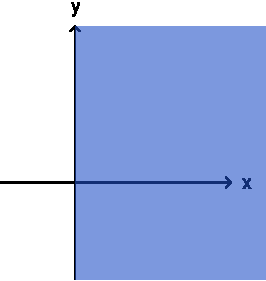
\includegraphics[scale=0.5]{cm7.pdf}
	\caption{En $x=0$ están los puntos frontera}
\end{figure}

Lo marcado en Azul, puede ser un conjunto llamado $A$ que $\forall(x,y)\in A\exists r<0\mid B\left((x,y),r\right)\subset A$

Si $(x,y)\in A$ por definición $x<0\implies$ Sea $r=x$, si $\left(x_1,y_1\right)\in B\left((x,y),r\right)\implies \left\lvert x_1-x\right\rvert=\sqrt{(x_1-x)^2}\leq \sqrt{(x_1-x)^2+(y_1-y)^2}<r=0$
\begin{equation*}
	\begin{cases}
		 & x_1-x<r=z \\
		 & x-z_1<r=x
	\end{cases}\implies x_1<r\implies x_1<0
\end{equation*}

Es decir que $(x_1,y_1)\in A\therefore B\left((x,y),r\right)\subset A$
Por lo tanto $A$ es un conjunto abierto

\begin{definition}[Sea $A\subset \R^n$]
	Un punto $X\in \R^n$ es un punto frontera del conjunto $A$ si para toda
	vecindad de $X$ contiene al menos un punto de $A$ y al menos un punto de fuera del conjunto $A$
\end{definition}

\section{Operación con funciones}

Se definen de forma análoga a como se hace en el caso de funciones univariadas. Considérese las funciones:
$f:I\subset \R^3\to \R$ y $V\subseteq \R^n\to \R$ se define:

\begin{enumerate}
	\item La suma diferencia de $f$ y $g$ como la función:
	      \begin{equation}
		      f\pm g:(U\cap V)\subseteq \R^n\to \R\mid (f+g)(x)=f(x)+g(x);\forall x\in\left(U\cap V\right)
	      \end{equation}
	\item El producto de $f$ y $g$ como la función:
	      \begin{equation}
		      f\cdot g:\left(U\cap V\right)\subseteq \R^n\to \R\mid \left(f(x)\cdot g(x)\right)(x)=f(x)\cdot g(x);\forall x\in\left(U\cap V\right)
	      \end{equation}
	\item El cociente de $f$ y $g$ como la función:
	      \begin{equation}
		      \frac{f}{g}:w\subseteq \R^n\to \R\mid \left(\frac{f}{g}\right)(x)=\frac{f(x)}{g(x)}\mid w=U\cap V-\left\{x\in V\mid g(x)=0\right\}
	      \end{equation}
\end{enumerate}

\begin{example}
	Dadas las funciones $f(x_a,x-2)=\sqrt{1-x_1^2-x_2^2}$ y $g(x_1,x_2)=\ln{(x_1\cdot x_2)}$ determinar:
	\begin{align*}
		 & (f+g)(x) &  & (f\cdot g)(x) &  & \left(\frac{f}{g}\right)(x)
	\end{align*}
\end{example}

\textit{ Sol. }

Se determinan los dominios de $f$ y $g$ para el dominio de $f:1-x_1^2-x_2^2\geq 0\implies 1\geq x_1^2+x_2^2$ al
considerar la igualdad asociada $x_1^2+x_2^2=1$, se observa que el dominio de $f$ es el disco unitario
con centro en (0,0).

\begin{equation*}
	Dom\, f=\left\{(x_1,x_2)\mid x_1+x_2\leq 1\mid x_1,x_2\in \R \right\}
\end{equation*}

Para el dominio de $g$, el logaritmo natural tiene sentido evaluarse cuando el argumento es positivo.
es decir:

\begin{align*}
	 & x_1\cdot x_2>0\longleftrightarrow x_1>0\land x_2>0 \\
	 & x_1\cdot x_2<0\longleftrightarrow x_1<0\land x_2>0
\end{align*}

Ahora, la intersección de $U$ con $V$ se vería como:

\begin{figure}[h!]
	\centering
	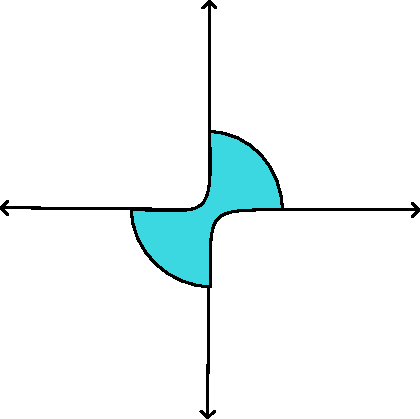
\includegraphics{cm8.pdf}
	\caption{$Dom\, g= \left\{(x_1, x_2)\right\}$}
\end{figure}

\begin{align*}
	 & (f+g)(x)=f(x)+g(x)=\sqrt{1-x_1^2-x_2^2}+\ln{(x_1\cdot x_2)}           \\
	 & (f\cdot g)(x)=f(x)\cdot g(x)=\sqrt{1-x_1^2-x_2^2}+\ln{(x_1\cdot x_2)}
\end{align*}

El dominio para las funciones $f+g$ y $f\cdot g$ se verá como:

\begin{equation*}
	Dom\, f+g=\left\{(x_1,x_2)\mid x_1^2+x_2^2\leq 1\land x_1\cdot x_1>0\mid x_1,x_2\in\R                                \right\}
\end{equation*}


\begin{example}
	Demuestre que $\lim_{(x,y)\to (1,3)}(2x+3y)=11$
\end{example}

\textit{ Sol. }

\textbf{Análisis preliminar: }
\begin{align*}
	 & \left\lvert f(x,y)-L\right\rvert =\left\lvert 2x+3y-11\right\rvert=\left\lvert (2x-2)+(3y-9)\right\rvert      \\
	 & =\left\lvert 2(x-1)+3(y-3)\right\rvert \leq \left\lvert 2(x-1)\right\rvert +\left\lvert 4(y-3)\right\rvert    \\
	 & =\left\lvert 2\right\rvert \left\lvert x-1\right\rvert +\left\lvert 3\right\rvert \left\lvert y-3\right\rvert \\
	 & \left\lvert x-1\right\rvert =\sqrt{(x-1)^2}\leq \sqrt{(x-1)^2+(y-3)^2}<\sigma                                 \\
	 & \left\lvert y-3\right\rvert =\sqrt{(y-3)^2}\leq \sqrt{(x-1)^2+(y-3)^2}                                        \\
	 & \left\lvert 2x-3y-11\right\rvert \leq 5\delta=\epsilon\implies \delta=\frac{1}{5}\epsilon
\end{align*}
\begin{proof}[$\forall \epsilon>0\exists\delta>0\, \left(\delta=\frac{1}{5}\epsilon\right)\mid 0<\sqrt{(x-1)^2+(y-3)^2}<\delta$]
	\begin{align*}
		 & \implies \left\lvert x-1\right\rvert <\delta \land \left\lvert y-3\right\rvert <\delta \\
		 & 2\left\lvert x-1\right\rvert +3\left\lvert y-3\right\rvert <5\delta                    \\
		 & \left\lvert 2(x-1)+3(y-3)\right\rvert <5\left(\frac{1}{5}\epsilon \right)              \\
		 & \therefore \left\lvert 2x+3y-11\right\rvert<\epsilon
	\end{align*}
\end{proof}

\begin{example}
	Demuestre que no existe:
	\begin{equation*}
		\lim_{(x,y)\to (0,0)}\frac{xy}{x^2+y^2}
	\end{equation*}
\end{example}

\textit{ Sol. }

\begin{figure}[h!]
	\centering
	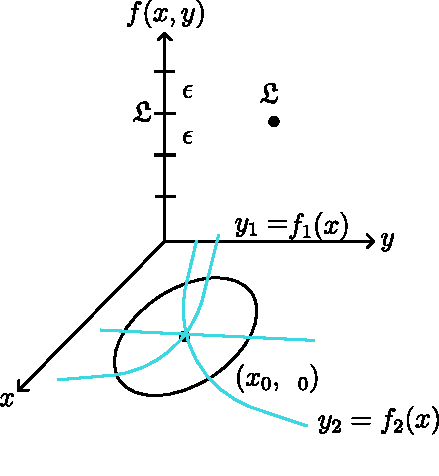
\includegraphics{cm9.pdf}
	\caption{Gráfica de cajas y ejes}
\end{figure}


\begin{align*}
	 & \lim_{x,y\to (0,0)}f(x,y)=\lim_{(x,y)\to (0,0)}f(x,x)=\lim_{x\to 0}\frac{x\cdot x}{x^2+x^2} \\
	 & =\lim_{x\to 0}\frac{x^2}{2x^2}=\lim_{x\to 0}\frac{1}{2}=\frac{1}{2}
\end{align*}

Como los límites son distintos por trayectorias distintas cuando se acercan al (0,0), se concluye que el límite no existe

\begin{align*}
	 & \lim_{(x,y,z)\to (0,0,0)}\frac{x+y+z}{x+y-z}=\lim_{(x,y,z)\to (0,0,0)} f(0,0,z)=                             \\
	 & \lim_{z\to 0}\frac{0+0+z}{0+0-z}=\lim_{z\to 0}\frac{z}{-z}=\lim_{z\to 0}-1=-1                                \\
	 & \lim_{(x,y,z)\to (0,0,0)}\frac{x+y+z}{x+y-z}=\frac{x+x+x}{x+x+x}=\lim_{x\to 0}\frac{3x}{x}=\lim_{x\to 0} 3=3
\end{align*}

\begin{theorem}[Unidad de los límites]
	Si $f:u\subseteq \R^n\to\R$, con $U$ conjunto abierto y si:
	\begin{equation*}
		\lim_{x\to x_0}m_1\, \lim_{x\to x_0}f(x)=m_2\implies m_1=m_2
	\end{equation*}
\end{theorem}

\begin{theorem}
	Sea $f$ y $g$ funciones $f:U\subset \R^n\to \R$ y
	$g:U\subseteq \R^n\to \R$
	y sea $X_0$ un punto en $u$ o en $\partial U$, además suponga que
	\begin{equation*}
		\lim_{x\to x_0}f(x)=\mathfrak{L}\land \lim_{x\to x_0}f(x)=\mathfrak{L}
	\end{equation*}

	Entonces:
	\begin{equation}
		L+M
	\end{equation}
	\begin{equation}
		\lim_{x\to x_0}(f\cdot g)(x)=\lim_{x\to x_0}f(x)\cdot \lim_{x\to x_0}g(x)=\mathfrak{L}\cdot M
	\end{equation}
	Siempre y cuando $M\neq 0$, entonces:
	\begin{equation}
		\lim_{x\to x_0}\left(\frac{f}{g}\right)(x)=\lim_{x\to x_0}f(x)
	\end{equation}
\end{theorem}

\begin{definition}
	Sean $U\subseteq \R$ un conjunto abierto y
	$f:U\subseteq \R^n\to \R$
	Entonces $\frac{\partial f}{\partial x},\frac{\partial f}{\partial x_2},\dots,\frac{\partial f}{ax_n}$ las derivadas parciales de $f$ respecto de la primera, segunda, $\dots$, n-+ésima variable son las funciones con valores reales
	de $n$ variables las cuales en el punto $X=\left(x_1,x_2,\dots,x_n\right)$ están definidas por:
\end{definition}
\begin{align*}
	 & \frac{\partial f}{ax_i}=\lim_{h\to 0}=\frac{f\left(x_1,x_2,\dots,x_i+h,\dots,x_n \right)-f\left(x_1,x_2,\dots,x_n \right)}{h} \\
	 & =\lim_{h\to 0}\frac{f(x+he_i)-f(x)}{h}
\end{align*}

\begin{example}
	Calcule $\frac{\partial f}{\partial c},\frac{\partial f}{\partial y}$ por medio de la definición para la función $f(x,y)=x^2y+xy^2$
\end{example}

\textit{ Sol. }

\begin{align*}
	 & \lim_{h\to 0}\frac{\left((x+h)^2y+(x+h)y^2\right)-\left(x^2y+xy^2\right)}{j}                             \\
	 & \lim_{h\to 0}\frac{x^2y+2xhy+h^2y+xy^2+hy^2x^2y-xy^2}{h}=\lim_{h\to 0}\frac{h\left(2xy+hy+y^2\right)}{h} \\
	 & \lim_{h\to 0}2xy+hy+y^2=2xy+y^2\implies \frac{\partial f}{\partial x}=2xy+y^2
	 & \frac{\partial f}{\partial y}=x^2+2xy
\end{align*}

\begin{example}
	Sea $f(x,y)=e{xy}$, mostrar que $x\frac{\partial f}{\partial x}=y\frac{\partial f}{\partial y}$
\end{example}

\textit{ Sol. }

\begin{align*}
	 & \frac{\partial f}{\partial x}=ye{xy}                                                     &  & \frac{\partial f}{\partial y}=xe{xy}                      \\
	 & x\cdot \frac{\partial f}{\partial x}=x\left(ye{xy}\right)                                &  & y\cdot \frac{\partial f}{\partial y}=y\left(xe{xy}\right) \\
	 & \implies x\frac{\partial f}{\partial x}=xye^{xy}=xye^{xy}=y\frac{\partial f}{\partial y}
\end{align*}

\begin{example}
	Evalúe la derivada parcial de $z=\ln{\sqrt{1+xy}}$ en los puntos (1,2) y (0,0)
\end{example}

\textit{ Sol. }

\begin{align*}
	 & \frac{\partial z}{\partial x}=\frac{1}{\sqrt{1+xy}}\cdot \frac{1}{2}(1+xy)^{-1/2}(y) \\
	 & \frac{\partial z}{\partial x}\mid_{1,2}=\frac{2}{2\left(1+(1)(2)\right)}=\frac{1}{3} \\
	 & \frac{\partial z}{\partial x}\mid_{0,0}=\frac{0}{2\left(1+(0)(0)\right)}=0           \\
	 & \frac{\partial z}{\partial y}=\frac{x}{2(1+xy)}\text{ Evaluando:}                    \\
	 & \frac{\partial z}{\partial y}\mid_{1,2}=\frac{1}{2\left(1+(1)(2)\right)}=\frac{1}{6} \\
	 & \frac{\partial z}{\partial y}\mid_{0,0}=\frac{0}{2\left(1+(0)(0)\right)}=0
\end{align*}

\begin{definition}
	Sea $f:U\subseteq \R^n\to \R;U$ conjunto abierto se define $Df(x)$ como el gradiente de $f$ en $x$ denotado por\footnote{$\nabla f(x)$ es un vector perpendicular a $f$ en $x$ que siempre apunta en la dirección de máximo (mínimo) crecimiento de $f$.}:
	\begin{equation}
		\nabla f(x)=\left(\frac{\partial f}{\partial x_1},\frac{\partial f}{\partial x_n},\dots,\frac{\partial f}{\partial x_n}\right)
	\end{equation}
\end{definition}

\section{Ecuación del plano tangente a una superficie}

Recordando la ecuación vectorial de un plano $\pi$ es:

\begin{equation}
	\overrightarrow{N}\cdot \left(X-X_0\right)=0
\end{equation}

Para el plano tangente $\pi_T$ en $X_0$ donde $x_0\in z=f(x,y)$
pero también es posible hacer lo siguiente (inmersión):
\begin{equation}
	\nabla f(X_0)\cdot \left(X-f(X_0)\right)=0
\end{equation}

\begin{align*}
	 & \left(\frac{\partial f}{\partial x}\mid_{x_0,y_0},\frac{\partial f}{\partial y}\right)\cdot \left((x,y)-(x_0,y_0)\right)=0                 \\
	 & \frac{\partial f}{\partial x}\left\lvert_{x,y} \left(x-x_0\right)+\frac{\partial f}{\partial y}\right\rvert_{(x0,y0)} \left(y-y_0\right)=0
\end{align*}

Para trasladarnos a la cuarta dimensión $ax+by+cz+d=0$:

\begin{align*}
	 & f(x,y)-z=0=G(x,y,z)\implies G(x,y,z)=f(x,y)-z \\
	 & \nabla G(X_0)\cdot \left(X-X_0\right)=0       \\
	 & X_0=\left(x_0,y_0,f(x_0,y_0)=x_0\right)
\end{align*}

Por lo tanto el gradiente de G:

\begin{align*}
	 & \nabla= G(x)=\left(\frac{\partial f}{\partial x},\frac{\partial f}{\partial y}-1\right)                                                              \\
	 & =\left(\frac{\partial f}{\partial x}\mid_{x_0,y_0},\frac{\partial f}{\partial y}\mid_{x_0,y_0}\right)\left((x,y,z)-\left(x_0,y_0,z_0\right)\right)=0 \\
	 & \frac{\partial f}{\partial x}\mid_{(x_0,y_0)}(x-x_0)+\frac{\partial f}{\partial y}\mid_{(x_0,y_0)}\left(y-y_0\right)-z+z_0=0
\end{align*}

Por lo tanto la ecuación del plano tangente será:

\begin{align*}
	z=\frac{\partial f}{\partial x}\mid_{x_0,y_0}\left(z-x_0\right)+\frac{\partial f}{\partial y}\mid_{x_0,y_0}\left(y-y_0\right)+f\left(x_0-y_0\right)
\end{align*}

\begin{example}
	Determine la ecuación del plano tangente a la superficie definido por $3xy+z^2=4$
	en el punto (1,1,1)
\end{example}

\textit{ Sol. }

Verificar que el punto (1,1,1) pertenezca a la superficie, es decir:
\begin{equation*}
	3(1)(1)+(1)^2=4=4
\end{equation*}
El punto (1,1,1) sí pertenece a la superficie.

Se supondrá que $G(x,y,z)=z^2+3xy-4=0$ y se procede como en la teoría.

\begin{align*}
	 & \frac{\partial G}{\partial x}\mid_{(1,1,1)}=3y &  & \frac{\partial G}{\partial y}\mid_{(1,1,1)}=3x &  & \frac{\partial G}{\partial z}\mid_{(1,1,1)}=-2z \\
	 & \frac{\partial G}{\partial x}\mid_{(1,1,1)}=3  &  & \frac{\partial G}{\partial y}\mid_{(1,1,1)}=3  &  & \frac{\partial G}{\partial z}\mid_{(1,1,1)}=-2
\end{align*}


\begin{equation*}
	\nabla G(1,1,1)=(3,2,2)
\end{equation*}

La ecuación del plano:

\begin{align*}
	 & (3,2,2)\cdot (x-1,y-1,z-1)=0                            \\
	 & 2x-3+3y-3+2z-2=0                                        \\
	 & 3x+3y+2z-8=0\implies \text{Ecuación del plano tangente}
\end{align*}

\begin{example}
	Use el plano tangente para hacer una aproximación local en el punto $(0,\frac{\pi}{6},1)$ para la función: $z=e^{3x}\sin{(3y)}$
\end{example}

\textit{ Sol. }

\begin{equation*}
	e^{3\cdot 0}\cdot \sin{2(\frac{\pi}{6})}=e^0\cdot \sin{\left(\frac{\pi}{2}\right)}=1\cdot 1=1
\end{equation*}
El punto sí pertenece a la superficie.

Se determina el plano tangente a la superficie en $(0,\frac{\pi}{6},1)$:
\begin{align*}
	 & G(x,y,z)=e^{3x}\cdot \sin{(3y)}-z=0                                                                                                   \\
	 & \nabla G(x,y,z)=\left(e^{3x}\cdot \sin{(3y)},e^{3x}\cdot \cos{(3y)},-1\right)                                                         \\
	 & \nabla G\left(0,\frac{\pi}{6},1\right)=\left(3e^{0}\cdot \sin{(\frac{\pi}{2})},3e^{0}\cdot \cos{\left(\frac{\pi}{2}\right)},-1\right) \\
	 & \nabla G\left(0,\frac{\pi}{6},1\right)=\left(3,0,-1\right)
\end{align*}

La ecuación del plano tangente será:

\begin{align*}
	 & \left(3,0,-1\right)\cdot \left(x-0,y-\frac{\pi}{6},z-1\right)=0 \\
	 & 3x+z-1=0                                                        \\
	 & z=3x+z+1=0
\end{align*}

Aproxime $z(0.1,0.54)$ usando el plano tangente

\begin{align*}
	z(0.1,0.54z=3(0.1)+1 \\
	z(0.1,0.54)=1.3      \\
\end{align*}

El valor real de $z$ en (0.1,0.54) es:
\begin{equation*}
	z(0.1,0.54)=e^{3(0.1)}\cdot \sin{(3\cdot0.54)}=1.34822513
\end{equation*}

\section{Derivada direccional}

\begin{definition}[Derivada direccional]
	Sea $f: u\subset \R^n\to \R$, donde $u$ es un conjunto abierto de $\R$ y sea $x_0\in u$.
	Sea $v\in \R^n$ un vector unitario dado. Se define la derivada de la función $f\in x_0$
	en la dirección del $v$, denotada por $\frac{\sigma f}{\sigma v}\left(x_0\right)$ siempre y cuando el límite exista como:
	\begin{equation}
		\lim_{h\to 0}\frac{f\left(x_0+hv\right)-f(x_0)}{h}
	\end{equation}
\end{definition}

\begin{example}
	Para la función $d(x,y,z)=xyz$ calcule la derivada direccional, en la dirección del vector $v=\left(\frac{1}{3},-\frac{2}{3}-\frac{2}{3}\right)$
\end{example}

\textit{ Sol. }

a definición dice:

\begin{align*}
	 & \lim_{h\to 0}\frac{f\left((x_0,y_0,z_0)+h(v_1,v_2,v_3)\right)-f\left(x_0,y_0,z_0\right)}{h}=                                                               \\
	 & \lim_{h\to 0}\frac{f\left(x_0+\frac{1}{3}h.y_0-\frac{2}{3}h,z_0-\frac{2}{3}h)\right)-x_0,y_0,z_0}{h}=                                                      \\
	 & \lim_{h\to 0}\frac{f\left(x_0+\frac{1}{3}h\right)\left(y_0-\frac{2}{3}h\right)\left(z_0-\frac{2}{3}h\right)-x_0,y_0,z_0}{h}=                               \\
	 & \lim_{h\to 0}\frac{\left(x_0y_0-\frac{2}{3}x_0h+\frac{1}{3}y_0h-\frac{2}{9}h^2\right)\left(z_0-\frac{2}{3}h\right)-x_0y_0z_0}{h}=                          \\
	 & \lim_{h\to 0}\frac{x_0y_0z_0-\frac{2}{3}x_0y_0h-\frac{2}{3}x_0z_0h+\frac{4}{9}x_0h^2+\frac{1}{3}y_0z_0h-\frac{2}{9}y_0h^2}{h}\dots                         \\
	 & \dots \frac{-\frac{2}{9}z_0h^2+\frac{4}{27}h^3-x_0y_0z_0}{h}=                                                                                              \\
	 & \lim_{h\to 0}\frac{h\left(-\frac{2}{3}x_0y_0-frac{2}{3}x_0z_0+\frac{4}{9}x_0h+\frac{1}{3}y_0z_0-\frac{2}{9}y_0h-\frac{2}{9}z_0h+\frac{4}{27}h^2\right)}{h} \\
	 & \lim_{h\to 0}-\frac{2}{3}x_0y_0-\frac{2}{3}x_0z_0+\frac{4}{9}x_0h+\frac{1}{3}y_0z_0-\frac{2}{9}y_0h-\frac{2}{9}z_0h+\frac{4}{27}h^2=                       \\
	 & -\frac{2}{3}x_0y_0-\frac{2}{3}x_0z_0+\frac{1}{3}y_0z_0=\frac{\partial f}{\partial v}\left(x_0,y_0\right)
\end{align*}

\begin{theorem}[a]
	Si $f:U\subset \R^n\to \R$ con $U$ un conjunto abierto de $\R^n$ y $f$ una función diferenciable, entonces existen todas las derivadas direccionales. La derivada direccional. La derivada direccional en $X$ en la dirección de $V$ está dada por:
	\begin{equation}
		\frac{\partial f}{\partial V}=\nabla f(x)\cdot V
	\end{equation}
	donde $V\in \R^n$
\end{theorem}

\begin{proof}
	Sea $l(h)=x+hV\mid l(0)=x\land l^{\prime}(0)=V$ por otro lado $f(x+hv)=f\left(l(h)\right)$ derivando ésta última expresión se tiene que:
	\begin{align*}
		 & f\left(l(h)\right)^{\prime}=f^{\prime}\left(l(h)\right)\cdot l^{\prime}(h)                    \\
		 & =\nabla f\left(l(h)\right)\cdot l^{\prime}(h)                                                 \\
		 & \frac{d}{dh}f(x+hv)=\nabla f\left(l(h)\right)\cdot l^{\prime}(h)                              \\
		 & \text{Evaluando la derivada en h=0 se tendría}                                                \\
		 & \frac{d}{dh}f(x+hv)\mid_{h=0}=\nabla f\left(l(0)\right)\cdot l^{\prime}(0)=\nabla f(x)\cdot V \\
		 & \frac{d}{dh}f(x+hv)\mid_{h=0}=\nabla f(x)\cdot v
	\end{align*}
\end{proof}

Empleando el teorema anterior, se tendría que:

\begin{align*}
	 & f(x,y,z)=xyz\, v=\left(\frac{1}{3},-\frac{2}{3},-\frac{2}{3}\right)                       \\
	 & \nabla f(x,y,z)=(yz,xz,xy)                                                                \\
	 & \nabla f(x,y,z)\cdot v=(yz,xz,xy)\cdot \left(\frac{1}{3},-\frac{2}{3},-\frac{2}{3}\right) \\
	 & =\frac{1}{3}yz-\frac{2}{3}xz+\frac{2}{3}xy
\end{align*}

\subsection{Regla de la cadena}

Si $U$ es una función diferenciable con variables independientes $x,y$ definida por
$U=f(x,y)$ donde $x=F(r,s)$ y $y=G(r,s)\implies$

\begin{align*}
	\frac{\partial U}{\partial r}=\frac{\partial U}{\partial x}\cdot \frac{\partial x}{\partial r}+\frac{\partial U}{\partial y}\cdot \frac{\partial y}{\partial r} \\
	\frac{\partial U}{\partial s}=\frac{\partial u}{\partial x}\cdot \frac{\partial x}{\partial s}+\frac{\partial U}{\partial y}\cdot \frac{\partial y}{\partial s}
\end{align*}

\begin{figure}[h!]
	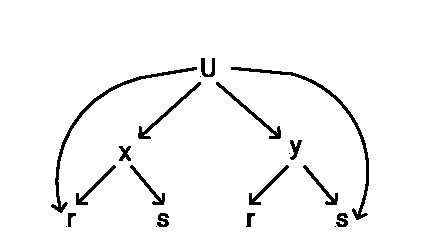
\includegraphics{cm10.pdf}
	\caption{Esquemáticamente}
	\label{cm10}
\end{figure}

\begin{example}
	i $f$ es una función diferenciable de las variables $u$ y $v$
	considere que $u(x,y)=x-y$ y $v(x,y)=x-y$ demuestre que
	$z=f(u,v)$ satisface la ecuación:
	\begin{equation*}
		\frac{\partial z}{\partial x}+\frac{\partial z}{\partial y}=0
	\end{equation*}
\end{example}

\textit{ Sol. }
\begin{align*}
	\frac{\partial z}{\partial x}=\frac{\partial z}{\partial u}\cdot \frac{\partial u}{\partial x}+\frac{\partial z}{\partial v}\cdot \frac{\partial v}{\partial x} \\
	\frac{\partial z}{\partial y}=\frac{\partial z}{\partial u}\cdot \frac{\partial u}{\partial y}+\frac{\partial z}{\partial v}\cdot \frac{\partial v}{\partial y}
\end{align*}
Por otro lado
\begin{align*}
	 & \frac{\partial u}{\partial x}=1  &  & \frac{\partial v}{\partial y\partial x}=-1 \\
	 & \frac{\partial u}{\partial y}=-1 &  & \frac{\partial v}{\partial y\partial y}1   \\
\end{align*}
Sustituyendo en $\frac{\partial z}{\partial x}$ y $\frac{\partial z}{\partial y}$

\begin{align*}
	\frac{\partial z}{\partial x}=\frac{\partial z}{\partial u}(1)+\left(\frac{\partial z}{\partial v}\right)(-1)=\frac{\partial z}{\partial u}+\frac{\partial z}{\partial v} \\
	\frac{\partial z}{\partial y}=\frac{\partial z}{\partial u}(-1)+\left(\frac{\partial z}{\partial v}\right)1=-\frac{\partial z}{\partial u}+\frac{\partial z}{\partial v}
\end{align*}
Así mismo las derivadas:
\begin{equation*}
	\frac{\partial z}{\partial x}+\frac{\partial z}{\partial y}=\left(\frac{\partial z}{\partial u}-\frac{\partial z}{\partial v}\right)+\left(-\frac{\partial z}{\partial U}+\frac{\partial z}{\partial v}\right)=0
\end{equation*}

%\begin{example}
%    Suponga que $W=f(x,y),\, x(r,\theta)=r\cos{(\theta)},\, y(r\theta)=r\sin{(\theta)}$. demuestre que:
%    \begin{equation*}
%        \left(\frac{\partial W}{\partial x}\right)^2+\left(\frac{\partial W}{\partial y}\right)^2=\left(\frac{\partial W}{\partial r}\right)^2+\frac{1}{r^2}\left(\frac{\partial W}{\partial \theta}\right)^2
%    \end{equation*}
%\end{example}
%
%\textit{ Sol. }

\subsection{Derivadas parciales de orden superior}

Ya se tiene definido cómo se determina una derivada
parcial de primer orden a la cual se denotará como

\begin{notation}
	\begin{equation*}
		\frac{\partial f}{\partial x}, \frac{\partial f}{\partial y},\dots
	\end{equation*}
\end{notation}

Una derivada parcial de segundo orden será:
\begin{align*}
	 & \frac{\partial\left(\frac{\partial f}{\partial x}\right)}{\partial x}=\frac{\partial^2f}{\partial x^2}; \frac{\partial\left(\frac{\partial f}{\partial y}\right)}{\partial y}=\frac{\partial^2f}{\partial y^2}                 \\
	 & \frac{\partial\left(\frac{\partial f}{\partial x}\right)}{\partial y}=\frac{\partial^2f}{\partial y\partial x}; \frac{\partial\left(\frac{\partial f}{\partial y}\right)}{\partial x}=\frac{\partial^2f}{\partial x\partial y}
\end{align*}
Si $f=f(x,y)$ es claro que $\frac{\partial f}{\partial x}=g(x,y)$
lo mismo que $\frac{\partial f}{\partial y}=h(x,y)$

\begin{example}
	Sea $h(x,y)=xye{xy}$ calcule todas las derivadas parciales de segundo orden de $h(x,y)$
\end{example}

\textit{ Sol. }

\begin{align*}
	 & \frac{\partial h}{\partial x}=ye^{xy}+xy^2e^{xy};\, \frac{\partial h}{\partial y}=xe^{xy}+x^2ye^{xy} \\
	 & \frac{\partial^2 h}{\partial^2 x}=y^2e^{xy}+y^2e^{xy}+xy^3e^{xy}=2y^2e^{xy}+xy^3e^{xy}
\end{align*}

\section{Extremos de funciones}

Caso de funciones de $\R^2\to \R$.

Sea $f:U\subseteq \R^n\to \R$ una función continua y diferenciable en $U$,
se dice que el punto $x_0\in U$ es un punto crítico de $f$ si

\begin{align*}
	 & \frac{\partial f}{\partial x}\mid_{x0}=0 &  & \frac{\partial f}{\partial y}\mid_{x0}=0
\end{align*}

O en todo caso cuando no existen.

\subsection{Clasificación de los puntos}

Los puntos crítico para ser clasificados como mínimo, máximo, punto silla
o no es un extremo o no es posible clasificar con éste criterio.

\begin{theorem}
	Sea $f:U\subseteq \R^2\to \R$ de clase $C^2$ en $U\subset \R$. Un punto
	$X_0=\left(x_0,y_0\right)$ es un mínimo local estricto de $f$ si se cumplen las tres condiciones siguientes:

	\begin{align}
		 & \frac{\partial f}{\partial x}\mid_{x0}=\frac{\partial f}{\partial y}\mid_{x_0}=0                                                                                                          \\
		 & \frac{\partial^2 f}{\partial x^2}\mid_{x_0}>0                                                                                                                                             \\
		 & \Delta (x_0)=\left(\frac{\partial^2}{\partial x^2}\mid_{x0}\right)\left(\frac{\partial^2}{\partial y^2}\mid_{x0}\right)-\left(\frac{\partial^2}{\partial x\partial y}\mid_{x0}\right)^2>0
	\end{align}
\end{theorem}

\begin{enumerate}
	\item Si en la segunda ecuación se tiene que es negativo (sin cambiar la condición tres) entonces el punto $X_0$ es un máximo local estricto de $f$.
	\item Si se cumlpe la primera y segunda, pero en la tercera ecuación cambia de sentido de igualdad ``<0'' implica que
	      el punto $X_0$ es un punto silla de $f$.
	\item No hay ningúna conclusión si en la tercera ecuación si $\Delta(x_0)=0$ (el criterio no funciona para clasificar el punto crítico)
\end{enumerate}

\begin{example}
	Dada la función $f:U\subset \R^2\to \R$, $f(x,y)=2x^4+y^2-x^2-2y$ determine
	y clasifique todos sus puntos extremos si es que existen.
\end{example}

\textit{ Sol. }

Primero se determinan los puntos críticos:
\begin{equation*}
	\frac{\partial f}{\partial x}=8x^3-2x=0\implies \frac{\partial f}{\partial y}=2y-2=0
\end{equation*}
Resolviendo el sistema de ecuaciones

\begin{align*}
	 & x\left(4x^2-1\right)=0 &  & y=1 \\
	 & x=0                    &  & y=1
\end{align*}
El punto crítico es $X_0=\left(0,1\right)$ o bien como $4x^2-1=0$
entonces $y=1$ y $x=\pm\frac{1}{2}$, con $y=1$. Por lo tanto se tienen otros dos puntos críticos:

\begin{align*}
	 & X_1=\left(-\frac{1}{2},1\right) &  & X_2=\left(\frac{1}{2},1\right)
\end{align*}

\textbf{Clasificación de los puntos críticos}

\begin{align*}
	 & \frac{\partial^2 f}{\partial x^2}=24x^2-2   &  & \frac{\partial^2 f}{\partial y^2}=2                          \\
	 & \frac{\partial^2 f}{\partial x\partial y}=0 &  & \frac{\partial^2 f}{\partial x^2}\mid_{(0,1)}=24(0)^2-2=-2<0
\end{align*}

\begin{align*}
	 & \frac{\partial^2 f}{\partial x^2}\mid_{\left(-\frac{1}{2},1\right)}=24\left(-\frac{1}{2}\right)^2-2=4>0 \\
	 & \frac{\partial^2 f}{\partial x^2}\mid_{\left(\frac{1}{2},1\right)}=24\left(\frac{1}{2}\right)^2-2=4>0
\end{align*}

Para el tercer criterio se realiza:

\begin{align*}
	\Delta (X_0)=(-2)(2)-(0)^2=-4<0
	\frac{\partial^2 f}{\partial y^2}\mid_{\left(0,1\right)}=2
\end{align*}
Evaluando (0,1) en la función, se tiene  como -1, entonces el punto (0,1,-1) $f$ tiene un punto silla.

Para el punto $x_1=\left(-\frac{1}{2},1\right)$:
\begin{align*}
	 & \frac{\partial^2 f}{\partial x^2}\mid_{\left(-\frac{1}{2},1\right)}=24\left(-\frac{1}{2}\right)^2-2=4 \\
	 & \frac{\partial^2 f}{\partial y^2}\mid_{\left(-\frac{1}{2},1\right)}=2                                 \\
	 & \Delta (X_1)=(4)(2)-(0)^2=8>0                                                                         \\
	 & \text{El punto }\left(-\frac{1}{2},1,-\frac{9}{8}\right)\text{ es un mínimo local estricto}           \\
	 & \text{El punto }X_3\left(\frac{1}{2},1,z\right)                                                       \\
	 & \frac{\partial^2 f}{\partial x^2}\mid_{\left(\frac{1}{2},1\right)}=4>0                                \\
	 & \Delta(X_2)=4(2)-(0)^2=8>0
\end{align*}
El punto $\left(\frac{1}{2},1,-\frac{9}{8}\right)$ es un mínimo local estricto.

\begin{example}
	Determine y clasifique los puntos críticos de la función $f(x,y)=x^2-xy^2-x+y$
\end{example}

\textit{ Sol. }

\begin{align*}
	 & \frac{\partial f}{\partial x}=2xy-y^2-1=0 \\
	 & \frac{\partial f}{\partial y}=x^2-2x+1=0
\end{align*}

Despejando ``$x$'' de la primera ecuación, se tiene que:
\begin{equation*}
	2xy=y^2+1\implies x=\frac{1}{2}y+\frac{1}{2y}\mid y\neq 0
\end{equation*}
Ésta última se sustituye en la ecuación dos:
\begin{align*}
	 & \left(\frac{1}{2}y+\frac{1}{2y}\right)^2-2\left(\frac{1}{2}y+\frac{1}{2y}\right)y+1=0 \\
	 & \frac{1}{4}y^2+\frac{1}{2}+\frac{1}{4y^2}-y^2-1+1=0                                   \\
	 & -\frac{3}{4}y^2+\frac{1}{4y^2}+\frac{1}{2}=0                                          \\
	 & -3y^4+1+2y^2=0\implies -3y^4+2y^2-1=0                                                 \\
	 & y^2=m\implies y^4=m^2                                                                 \\
	 & m=\frac{-2\pm\sqrt{4-4(-3)(1)}}{-6}\implies \begin{cases}
		                                                & m_1=1 \\&m_2=-\frac{1}{3}
	                                               \end{cases}
\end{align*}
Pero como $y^2=m\implies y^2=1\land y^2=-\frac{1}{3}$
las únicas soluciones son $y\pm 1$, sustituyendo estos valores en la expresión para $x$, se obtiene para $y=1$:
\begin{equation*}
	x=\frac{1}{2}(1)+\frac{1}{2(1)}=1
\end{equation*}
Con ésto se tiene el punto crítico $P_0=(1,1)$
Para $y=-1$:
\begin{equation*}
	x=\frac{1}{2}(-1)+\frac{1}{2(-1)}=-1
\end{equation*}
Con ésto se tiene el punto crítico $P_1=(-1,-1)$

\begin{align*}
	\frac{\partial^2 f}{\partial x^2}=2y &  & \frac{\partial^2 f}{\partial y^2}=-x &  & \frac{\partial^2 f}{\partial x\partial y}=2x-2y
\end{align*}

Considerando el punto crítico $P_0=\left(1,1\right)$ para su clasificación:

\begin{equation*}
	\frac{\partial^2 f}{\partial x^2}\mid_{(1,1)}=2(1)=2>0
\end{equation*}

\begin{align*}
	 & \Delta(1,1)=(2)(-2)-\left(2(1)-2(1)\right) \\
	 & \Delta(1,1)=-4<0
\end{align*}
La conclusión es que el punto crítico $P_0=(1,1,0)$ la función $f$
tiene un punto silla.

Se repite el análisis para el punto crítico $P_1=(-1,-1,0)$

\begin{equation*}
	\frac{\partial^2 f}{\partial x^2}\mid_{(-1,-1)}=2(-1)=2>0
\end{equation*}

\begin{align*}
	 & \Delta(-1,-1)=(-2)(2)-(0)^2 \\
	 & \Delta(-1,-1)=-4>0
\end{align*}

Se concluye que para el punto crítico $P_1=(-1,-1,0)$ la función $f$
tiene un punto silla.


